% !TEX program = xelatex
\documentclass[UTF8,fontset=fandol,openany,11pt]{ctexbook}

\usepackage[a5paper,top=20mm,bottom=22mm,inner=21mm,outer=17mm,headheight=14pt]{geometry}
\usepackage{fontspec}
\usepackage{amsmath,mathtools}
\usepackage{unicode-math}
\setmainfont{texgyrepagella-regular.otf}[
  BoldFont=texgyrepagella-bold.otf,
  ItalicFont=texgyrepagella-italic.otf,
  BoldItalicFont=texgyrepagella-bolditalic.otf
]
\setsansfont{texgyreheros-regular.otf}[
  BoldFont=texgyreheros-bold.otf,
  ItalicFont=texgyreheros-italic.otf
]
\setmonofont{lmmono10-regular.otf}
\setmathfont{texgyrepagella-math.otf}

\usepackage{microtype}
\usepackage{setspace}
\setstretch{1.28}
\setlength{\parindent}{2em}
\setlength{\parskip}{0.15em}
\setlength{\emergencystretch}{3em}

\usepackage{booktabs,longtable,tabularx,array,multirow}
\usepackage{enumitem}
\setlist{nosep,leftmargin=2em}
\usepackage{xcolor}
\definecolor{deepblue}{HTML}{173B57}
\definecolor{warmgray}{HTML}{F3F1EC}
\definecolor{accent}{HTML}{9A5A36}
\usepackage[most]{tcolorbox}
\tcbset{enhanced,breakable,boxrule=.45pt,arc=1.2mm,left=1.5mm,right=1.5mm,top=1.2mm,bottom=1.2mm}
\newtcolorbox{learninggoals}{title=学习目标,colback=warmgray,colframe=deepblue,fonttitle=\bfseries}
\newtcolorbox{keypoint}{title=关键辨析,colback=blue!3,colframe=deepblue,fonttitle=\bfseries}
\newtcolorbox{workedexample}[1][]{title={完整算例：#1},colback=blue!3,colframe=deepblue,fonttitle=\bfseries}
\newtcolorbox{failurecheck}[1][]{title={失败诊断：#1},colback=red!2,colframe=accent,fonttitle=\bfseries}
\newtcolorbox{chapterreview}{title=本章小结,colback=warmgray,colframe=accent,fonttitle=\bfseries}
\newtcolorbox{selfcheck}{title=自测与研讨,colback=white,colframe=accent,fonttitle=\bfseries}

\usepackage{tikz}
\usetikzlibrary{arrows.meta,positioning,fit,calc,shapes.geometric}
\tikzset{
  causalnode/.style={draw=deepblue,thick,circle,minimum size=8mm,inner sep=1pt},
  causalbox/.style={draw=deepblue,rounded corners,align=center,minimum height=8mm,fill=blue!3},
  causalarrow/.style={-{Latex[length=2mm]},thick,deepblue}
}

\usepackage{csquotes}
\usepackage[backend=biber,style=gb7714-2015ay,gbpub=false,maxcitenames=2,mincitenames=1,sorting=nyt,doi=true,url=true,isbn=false]{biblatex}
\DeclareLanguageMapping{english}{english}

% Keep index generation under latexmk so out-of-tree builds remain reproducible.
\usepackage{makeidx}
\usepackage{fancyhdr}
\usepackage{emptypage}
\pagestyle{fancy}
\fancyhf{}
\fancyhead[LE]{\small\thepage\quad\leftmark}
\fancyhead[RO]{\small\rightmark\quad\thepage}
\renewcommand{\headrulewidth}{0.3pt}
\fancypagestyle{plain}{\fancyhf{}\fancyfoot[C]{\thepage}\renewcommand{\headrulewidth}{0pt}}

\usepackage{titlesec}
\titleformat{\chapter}[display]
  {\sffamily\bfseries\color{deepblue}}
  {\filleft\Large 第\thechapter 章}
  {0.8ex}
  {\titlerule\vspace{1ex}\Huge}
\titleformat{name=\chapter,numberless}[display]
  {\sffamily\bfseries\color{deepblue}}{}{0pt}{\titlerule\vspace{1ex}\Huge}
\titleformat{\section}{\Large\sffamily\bfseries\color{deepblue}}{\thesection}{0.7em}{}
\titleformat{\subsection}{\large\sffamily\bfseries\color{accent}}{\thesubsection}{0.7em}{}

\usepackage{hyperref}
\hypersetup{
  unicode=true,
  colorlinks=true,
  linkcolor=deepblue,
  citecolor=accent,
  urlcolor=deepblue,
  pdftitle={因果推理深度读本}
}
\usepackage[nameinlink,noabbrev]{cleveref}

\newcommand{\term}[1]{\textbf{#1}\index{#1}}
\newcommand{\eng}[1]{\textit{#1}}
\newcommand{\doop}{\operatorname{do}}
\newcommand{\indep}{\mathrel{\perp\!\!\!\perp}}
\newcommand{\chapterreadings}[1]{\section*{延伸阅读}\addcontentsline{toc}{section}{延伸阅读}\begin{sloppypar}#1\end{sloppypar}}

\addbibresource{references.bib}
\makeindex

\title{因果推理深度读本\\\large 从哲学问题到现代形式方法}
\author{}
\date{}

\begin{document}

\frontmatter
\maketitle
\input{chapters/frontmatter-preface}
\input{chapters/frontmatter-guide}
\tableofcontents

\mainmatter

\part{因果概念、历史与哲学}
\input{chapters/chapter-01-questions}
\input{chapters/chapter-02-history}
\chapter{当代因果哲学：反事实、概率、机制与干预}
\label{ch:philosophies}

\begin{learninggoals}
读完本章，你应当能够：比较反事实、概率、机制、能力与干预理论的分析对象；检验先占、过度决定、遗漏和共同原因等反例；说明多元证据怎样形成受约束的整合，而非概念拼贴。
\end{learninggoals}

\section{反事实因果：刘易斯及其难题}

\subsection{反事实语义、依赖与因果链}

日常判断原因时，我们自然会问：“如果原因没有发生，结果还会发生吗？”若苏茜投出的石块击碎玻璃，而没有这次投掷玻璃便不会碎，我们倾向于把投掷视为原因。这个\term{若无检验}（\eng{but-for test}）抓住了原因作为差异制造者的直觉，并给出因果方向：结果依赖原因，原因通常不以同样方式依赖结果。
困难在于反事实前件与事实相反。我们不能简单查看实际数据中“同一个对象同时未受处理”的结果，也不能只用材料蕴涵，因为一个前件为假的材料条件句会自动为真。反事实理论需要说明：在保留多少实际背景的前提下，怎样评价“若 $A$ 未发生，$C$ 会怎样”。

\paragraph{可能世界与相似性}

\textcite{lewisCounterfactuals}以可能世界之间的比较相似性给出反事实语义。常用的直观说法是：考察与现实最相似的 $A$ 世界，若相关的最相似 $A$ 世界都是 $C$ 世界，则“若 $A$，则 $C$”为真。但Lewis并不要求必须存在一个或一组“最近的 $A$ 世界”；他明确拒绝这种\term{极限假设}（limit assumption）。在不假定最近世界存在的更一般表述中，只要存在 $A$ 世界，“若 $A$，则 $C$”为真可理解为：有某个 $A\land C$ 世界比任何 $A\land\neg C$ 世界都更接近现实。因此，“最接近世界”适合作直观入口，却不应被读成Lewis正式语义必须满足的存在性条件。
这里的世界不是平行宇宙的经验假说，而是评价模态命题的理论装置。世界之间的“接近”也不是表面相似度的简单加总，而由受语境与自然规律约束的比较相似性排序决定。

评价“若火柴没有被划，是否会燃烧”时，我们通常允许一个小的局部偏离使划火柴事件不发生，同时尽可能保留现实规律和广泛事实。若为了保持更多局部事实而允许大规模违反规律，反事实判断会失去稳定性。Lewis在讨论因果时给予避免巨大、广泛奇迹较高优先级，再考虑事实吻合范围。
相似性语义的优点是能够处理非因果反事实，并解释为何“回溯式”反事实通常不成立。例如，若结果没有发生，我们通常不会反推原因也未发生，而倾向于假定因果过程在原因之后出现局部偏离。但相似性排序本身也受到批评：若我们已经凭因果判断决定哪些世界更接近，再用接近关系定义因果，就可能产生循环。

\paragraph{从反事实依赖到因果链}

Lewis早期分析把事件理解为时空区域中具有特定性质的个体。若 $c$ 和 $e$ 都实际发生，且
\[
\neg O(c)\xRightarrow{\mathrm{cf}} \neg O(e),
\]
即在最接近的无 $c$ 世界中也没有 $e$，则 $e$ 对 $c$ 存在\term{因果依赖}\parencite{lewisCausation1973}。这里 $O(c)$ 表示事件 $c$ 发生。

简单依赖并不总是传递。若按下开关导致继电器动作，继电器动作导致灯亮，我们希望开关是灯亮的远因，即使某些复杂背景使端点之间的直接反事实依赖失败。Lewis因此把因果关系定义为因果依赖链的祖先关系：存在事件序列 $c,d_1,\dots,e$，每个后项因果依赖前项。
这一做法恢复了因果传递性，却也制造过度传递问题。一个人向右躲开巨石，因此恰好站到后来被树枝击中的位置；躲避依赖巨石，受伤依赖躲避，但说巨石造成树枝击伤可能很勉强。是否传递取决于我们追踪的是能量过程、机会条件，还是与问题相关的变量路径。

\subsection{先占、过度决定与遗漏难题}

\term{早期先占}的经典例子中，苏茜和比利都向瓶子投石。苏茜的石块先击中并打碎瓶子，比利的石块稍后到达原位置。苏茜是实际原因，比利只是备份。然而，若苏茜没有投掷，比利仍会打碎瓶子，所以“没有苏茜投掷，瓶子不会碎”为假。简单若无检验遗漏了苏茜这个原因。

因果链方法可以区分实际过程：苏茜投掷经由飞行、撞击和裂纹形成到达破碎；比利链条在撞击前被截断。但\term{晚期先占}更困难：两条过程可以延伸很远，直到后期一个过程阻止另一个。要指出“哪条链是实际链”，理论往往需要对过程结构作比简单端点反事实更细的描述。

\term{对称过度决定}中，两枚同时且各自足够的炸弹共同摧毁目标。没有任意一枚，另一枚仍足够，因而两者都不通过若无检验；直觉却把两者都视为原因。可以把检验改成“在适当背景或某个事件子集中，改变该因素会改变结果”，但何谓适当背景必须防止任意挑选。

\paragraph{从是否发生到如何发生}

Lewis后期提出\term{因果影响}分析。一个事件 $c$ 影响事件 $e$，不是只要求“无 $c$ 则无 $e$”，而是要求 $c$ 的一系列细微变化与 $e$ 的一系列变化之间存在系统反事实对应\parencite{lewisInfluence2000}。投石时间、速度或方向的变化会改变玻璃破碎的时间、方式或碎片分布；即使备份原因保证“最终仍破碎”，实际结果的具体方式仍受苏茜投掷影响。
这一修正把二值发生扩展为事件的时间和方式，使先占案例更可处理。它仍依赖恰当的事件变更和相似性排序，也可能在微小改变引发复杂连锁时过宽。值得注意的是，《作为影响的因果》发表于2000年，而非有些二手资料误记的1986年。

\paragraph{遗漏、双重防止与规范背景}

“园丁没有浇水导致植物死亡”把一个缺席当作原因。若事件是时空中的具体个体，缺席似乎不是可进入因果链的事件；若允许一切缺席成为原因，则任何未发生的救援都可能被说成结果原因。我们通常依赖职责、常规或期待筛选相关遗漏：受雇园丁的不浇水比陌生人的不浇水更容易被视为原因。

\term{双重防止}也挑战简单过程直觉：保镖阻止刺客阻止解药送达，因而保镖的行动使解药到达。反事实上，保镖行动与获救存在依赖，但两者之间未必有从原因向结果传递的连续物理过程。反事实理论能自然容纳这类“让某过程不受阻”的因果，纯能量传递理论则较困难。

这些案例表明，实际因果判断可能同时依赖反事实结构、过程连接、事件描述粒度与正常性规范。结构因果模型中的实际因果定义尝试把这些要素形式化，但不同定义在先占、投票、法律责任等案例上仍有分歧。

\subsection{因果类型、事件粒度与证据来源}

“吸烟导致肺癌”通常是\term{类型因果}命题，涉及人群中的暴露分布与风险变化；“张某的吸烟导致了他的肺癌”是\term{个例因果}命题。前者可由试验、观测设计和机制证据支持，后者还需评价该个体的替代历史与实际过程。群体平均效应为零并不排除对不同亚组存在方向相反的作用，平均效应为正也不自动确定每一患者的实际原因。
现代政策评估大多以类型因果效应为目标；法律、历史和故障诊断则频繁提出个例因果问题。选用框架时应先看查询，而不是假定所有因果句都由同一个若无条件定义。

\paragraph{深读案例：委员会投票与结构敏感性}

五人委员会以至少三票通过提案，实际五人都投赞成。对任一成员，若只有他改投反对，提案仍通过，所以简单若无检验不把任何一票视为原因。若允许把其他两票设为反对作为应急背景，则某一票会成为关键；同样推理又把每票都算作原因。
这是否正确取决于查询。若问每位成员是否参与形成充分多数，全部赞成票都有贡献；若问谁的改变本可阻止提案，单独没有人；若问法律责任，职务、信息和串谋可能改变答案。结构模型需要明确聚合规则和应急情形，不能用一个“实际原因”标签消除问题差异。
再设主席只在平票时投票，实际普通成员三比一通过，主席未投票。主席的缺席不是提案通过的原因；但制度规则允许他的潜在票在其他背景中关键。这里必须区分因果能力、实际贡献和制度权力。反事实理论若不限定实际过程，可能把广泛备份能力误作具体原因。

\paragraph{事件描述粒度}

“苏茜投石”可以描述为一次具体肌肉动作、石块以某速度离手、石块击中某位置，或更抽象的“有人投掷”。反事实依赖会随描述变化。若苏茜没有以每秒十米速度投掷，她可能以九米速度投掷，瓶子仍碎；若她完全没有投掷，比利会接替。粗细粒度决定哪些替代世界最接近。
结果描述也一样。“瓶子碎了”在备份存在时不依赖苏茜，但“瓶子在12点00分以这种裂纹碎裂”可能依赖。后期影响理论利用这种细节，但过细结果会使几乎任何微小背景都成为原因。适当粒度应由解释问题决定，并保持在相似案例中一致，而不是为了得到直觉答案临时调整。
结构方程把事件粒度转化为变量选择。二元变量适合某些责任规则，过程变量适合先占路径。模型比较应说明新增变量如何对应真实过程及可获得证据，而非只证明“存在一幅图能给出想要答案”。

\paragraph{反事实判断的证据来源}

我们无法直接观察反事实，却可由多类证据约束。重复试验估计类型层面的干预差异；机制知识说明改变如何传播；时间与物理连续性识别实际路径；相似案例支持背景稳定；制度规则规定哪些替代情形可行。个例因果判断通常综合这些来源。
例如判断药物是否导致某患者过敏，群体试验显示风险提升，免疫检测显示特异机制，给药后时间吻合，停药后症状缓解，再暴露后复发。任何单项证据都可能不足，组合则强化“若无给药便无此次反应”的模型。反事实不是纯粹想象，而是受实际证据约束的模型推论。

\section{概率、机制、力量与干预：多元因果理论}

\subsection{概率、共同原因与INUS条件}

反事实理论突出差异制造，却可能难以刻画实际过程；规律论说明事件类型的稳定联系，却容易遗漏方向；机制论展示结果如何产生，却未必给出效应大小；概率理论适合不确定系统，却必须处理混杂；干预主义连接实验实践，却需要说明何种变化算合格干预。二十世纪后半叶的因果哲学由此呈现多元格局。
多元不等于所有理论都同样正确，也不意味着同一句因果话语可以任意解释。较稳妥的看法是：科学中的因果概念承担若干彼此相关的功能------预测操纵结果、解释生成过程、支持迁移、归属责任。不同理论把其中某一种功能当作分析中心。评价它们时，应同时问理论处理何种对象、服务何种查询、依赖何种背景。

\paragraph{概率提升与共同原因}

在随机或不完全观测系统中，原因不必保证结果。吸烟者并非人人患肺癌，未吸烟者也可能患病。概率因果理论据此把原因理解为提高结果概率的因素。最简单形式是
\[
P(E\mid C)>P(E\mid \neg C).
\]
Suppes把时间优先和概率提升结合起来讨论“表面原因”与“真正原因”\parencite{suppes1970}。

简单概率提升面临三类困难。第一是\term{混杂}：冰淇淋销售与溺水同时上升，是炎热天气共同影响二者，并非购买冰淇淋使人溺水。第二是\term{辛普森反转}：总体概率提升可能在每个相关亚组中消失或反向。第三是\term{预防原因}：安全带对死亡具有负向因果作用，表现为降低而非提高概率。因而更一般的语言应谈论概率改变，并要求在恰当背景中比较。

Reichenbach的\term{共同原因原则}指出：若两个事件相关，且彼此不是原因，则应寻找一个共同原因，使相关在适当条件下被“筛除”\parencite{reichenbach1956}。在简单情形中，若 $C$ 是 $A$ 与 $B$ 的共同原因，可期待
\[
P(A,B\mid C)=P(A\mid C)P(B\mid C).
\]
现代图模型把这种思想推广为条件独立结构，但共同原因原则不是无条件定理。选择偏差、确定关系、量子相关和不完整变量描述都会使简单筛除形式需要修正。

\paragraph{Mackie的INUS条件}

现实结果常由原因复合产生。电路短路并非任何情况下都引起火灾；它可能需要可燃物、氧气和保护装置失效共同出现。Mackie把许多日常原因分析为\term{INUS条件}：一个不充分但为某个不必要而充分条件之必要部分\parencite{mackie1974}。

设火灾 $F$ 可以由两组条件产生：
\[
(S\land O\land D)\lor(L\land G)\longrightarrow F,
\]
其中 $S$ 为短路，$O$ 为有氧环境，$D$ 为保护失效；另一条路径由雷击 $L$ 与干燥 $G$ 构成。$S$ 单独不足以导致火灾，但在组合 $S\land O\land D$ 中不可缺；这个组合足以导致火灾，却不是必要的，因为还有另一条路径。因此 $S$ 是 $F$ 的一个INUS条件。

INUS分析有两项贡献。它避免要求单一原因既必要又充分，并突出因果场景与替代充分集合。但形式中的“充分”通常相对于背景和模型，而非宇宙中绝对无例外；如何选择正常背景、如何处理概率结果和连续变量，也不是析取范式本身能够解决。INUS更像揭示复合原因结构的分析工具，而不是完整的因果形而上学。

\paragraph{Salmon：解释必须进入因果网络}

Salmon反对把科学解释仅仅看成定律下的推导。他早期使用统计相关模型，后来发展\term{因果过程}理论：能够传递结构或“标记”的过程，与只呈现运动轨迹的伪过程不同\parencite{salmon1984}。一束光可以携带调制信息；墙上的光斑可以超光速移动，却没有一个物体或信号沿光斑轨迹传播。
因果过程在交互中改变并把变化继续传递。两辆汽车碰撞后速度和形变改变，交互把此前过程连接到此后过程。解释一个事件，就是说明它如何嵌入产生它的因果网络，而不是仅仅展示一个包含它的统计规律。
“标记传递”后来受到批评：什么算可传递标记可能依赖反事实，难以覆盖场、持续约束和非局部结构。Salmon转向以守恒量传递刻画因果过程，但这更适合物理情形，对社会制度和生物调控未必直接适用。其核心遗产不是某个永恒定义，而是解释相关性要求追踪实际产生结构。

\subsection{机制、因果力量与干预主义}

生命科学中的机制解释通常不要求一条单独守恒量链，而把机制理解为实体和活动以特定时空方式组织并产生现象。Machamer、Darden与Craver强调“实体做什么”，Glennan则强调部件相互作用形成稳定行为\parencite{mdc2000,glennan2017}。
以动作电位为例，完整机制涉及膜、电压门控离子通道、离子浓度梯度以及通道依时间开闭的组织。仅说刺激与放电相关不能解释波形如何产生；仅列出部件也不够，必须说明活动顺序和组织。机制模型往往是多层且不完整的：研究目的决定需要向下分解到何种程度。
机制证据对外推尤其重要。若某药物在试验人群中有效，而目标人群缺少关键受体，平均效应未必可迁移。不过，机制叙述也可能只是“故事”。可靠机制解释需要独立测量、干预部件、追踪中间过程并排除竞争路径。

\paragraph{因果力量与能力}

Cartwright批评把自然定律视为处处无条件成立的普遍概括。实验定律常描述精心隔离的情形；现实结果由多种\term{因果能力}共同作用\parencite{cartwright1989}。阿司匹林具有缓解疼痛的能力，并不意味着每次服用都实际止痛，因为剂量、吸收、病因和其他药物会改变表现。
力量或能力语言抓住了原因在不同背景中仍可被识别的倾向性，也说明效应不是裸相关。但它面临测量和判准问题：若我们只通过效果知道某物有能力，再用能力解释效果，便有循环危险。实际科学需要通过多种独立表现、机制和干预来校准能力归属。

\paragraph{Woodward：不变性与干预}

Woodward的\term{干预主义}不把因果简化为人类实际能够操纵的东西，而是用理想干预定义变量层面的因果关系\parencite{woodward2003}。粗略地说，若存在对 $X$ 的合格干预，改变 $X$ 会改变 $Y$，则 $X$ 是 $Y$ 的原因之一。合格干预 $I$ 应改变 $X$，并且除经由 $X$ 外不通过其他路径直接影响 $Y$；它还应切断 $X$ 与其通常原因的联系。

这种要求可以用图表示：

\begin{center}
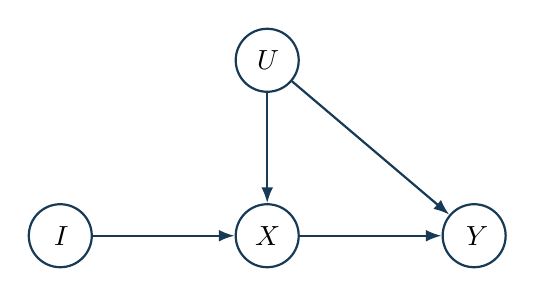
\begin{tikzpicture}[node distance=14mm and 18mm]
\node[causalnode] (i) {$I$};
\node[causalnode,right=of i] (x) {$X$};
\node[causalnode,right=of x] (y) {$Y$};
\node[causalnode,above=of x] (u) {$U$};
\draw[causalarrow] (i)--(x);
\draw[causalarrow] (x)--(y);
\draw[causalarrow] (u)--(x);
\draw[causalarrow] (u)--(y);
\end{tikzpicture}
\end{center}

理想干预使 $I$ 只通过 $X$ 影响 $Y$，并替代 $U\rightarrow X$ 的通常生成方式。随机试验是实现这种结构的一种设计，但干预主义也评价不可实际操作的变量：只要能够清楚定义合适的反事实改变，例如地壳运动或恒星质量，就可以讨论其因果影响。
Woodward还以\term{不变性}说明解释深度。一条关系若在多种针对输入的干预下保持稳定，就比只在狭窄数据范围内拟合良好的相关式更具有因果解释力。温度计读数与温度稳定共变，但直接改变温度计指针不会改变环境温度，显示关系方向不是由回归对称性决定。
干预定义会否循环？要判断 $I$ 不通过其他路径影响 $Y$，似乎已经使用因果概念。Woodward的回应不是把所有因果词还原为非因果词，而是提供相互约束的网络分析：变量关系、干预条件与不变性共同澄清科学实践中的因果主张。这是一种非还原分析，而非传统意义上的概念消除。

\subsection{理论互补、解释层级与选择准则}

以药物安全为例，概率数据说明药物如何改变不良事件风险；潜在结果或图模型说明在何种设计下该变化可归因于药物；机制研究追踪代谢与受体通路；能力语言描述药物在不同背景中的倾向；实际因果分析判断某病例的不良事件是否由药物造成。这些答案不能相互代替，却可以形成证据链。
理论多元的纪律在于明确接口：机制知识如何转化为图结构假设？概率效应在哪些背景中保持？干预改变的是机制中的哪个环节？个例归因是否有群体数据与过程证据支持？只有回答这些接口问题，多种理论才是互补；否则“综合”只是把不同术语并列。

\paragraph{贯穿案例：医院内感染}

某医院发现中心静脉导管患者血流感染率升高。概率理论首先比较置管与未置管风险，但病情严重者更可能置管，简单概率提升包含适应证混杂。潜在结果与图模型要求定义“在符合置管条件者中采用某种导管策略”的效应，并调整病情等共同原因。
机制调查追踪皮肤菌群、置管过程、导管表面生物膜和免疫反应。它解释为何无菌操作、敷料和拔管时机可能改变风险。INUS分析可把“导管存在、无菌屏障破坏、足够留置时间、易感宿主”视为一条充分条件组合；另一条感染路径可能来自远处感染播散。没有哪个因素单独必要充分。
因果能力语言说导管表面具有支持生物膜的倾向，但这种能力在涂层、抗菌措施和宿主不同条件下表现不同。干预主义要求检查改变导管材料、操作规范或留置时间是否系统改变感染，并区分这些可控变量的路径。实际病例归因还要判断培养结果、时间与替代来源。

这个案例显示，证据不是简单投票。若观察关联强但机制检测显示主要病例菌株来自另一来源，因果解释需修订；若机制在实验室成立但医院随机改进措施无效果，可能是实施失败、机制贡献太小或替代路径补偿。不同证据之间的冲突用于诊断模型，而非选择自己偏好的理论。

\paragraph{解释层级与干预层级}

医院可以在分子、设备、操作人员、病房和制度层面干预。同一结果具有多层原因：材料属性影响附着，护士工作负荷影响无菌操作，采购制度影响材料选择。低层机制不一定使高层因果失真；若改变排班稳定改变感染，高层变量具有政策相关的干预意义。
层级之间可能出现实现关系。工作负荷通过多种具体动作影响感染，不存在一个固定微观中介；要求把政策效应完全还原为每次手部动作才算“真正因果”，会让有用的宏观解释失效。反过来，高层标签若无法对应任何稳定实施方式，效应也难迁移。
因果多元主义由此不是给每层一个互不相干真理，而是要求跨层约束：宏观干预改变哪些机制分布，微观机制为何汇总成观察效应，背景变化如何改变实现。机制、概率和干预关系在这些接口上互相检验。

\paragraph{理论选择的实用准则}

如果目标是政策净效果，优先明确处理策略与人群平均反事实；如果目标是故障诊断，优先追踪实际过程和部件；如果目标是风险预警，概率关系可以在不承担干预解释时发挥作用；如果目标是迁移，机制与不变性尤为关键；如果目标是责任，需在实际因果之外加入规范标准。
同一项目可随阶段改变工具：探索阶段以概率和发现算法缩小假设，验证阶段以试验识别差异，解释阶段分解机制，部署阶段检验环境不变性。理论的价值由它对具体查询的约束力衡量，而不是由它能否把所有因果语言压成一句定义衡量。

\section{理论选择、证据整合与模型责任}

\subsection{用反例检验理论}

因果理论的差异只有放入困难案例才会清楚。先占案例中，两条潜在路径都足以产生结果，但其中一条先完成过程；简单若无检验可能把被截断的备份也算原因。对称过度决定中，两项因素同时足以，删除任一项结果仍发生，若无条件又把两个直觉原因都排除。遗漏案例中，不行动可能是结果的原因，却难以用能量传递描述。共同原因案例则提醒概率提升可以由上游因素制造。

检验理论时应逐项记录它改变了什么。刘易斯式方案可能修改事件描述、引入因果链或采用影响关系；机制论可能要求追踪实际过程；结构模型可能加入应急情形和正常性排序；概率理论可能条件化背景集合。修正解决一个反例时，往往同时增加新的理论负担。例如加入正常性有助于区分园丁浇水与植物存活，却需要解释正常判断来自统计、功能还是规范。

反例不必迫使所有理论竞争一个定义。若研究任务是分配法律责任，实际因果和规范背景不可避免；若任务是估计药物平均效应，个例正常性可能不是主要对象；若任务是解释细胞过程，机制组织比总体风险差更重要。真正需要统一的是同一任务中的概念使用，而不是把所有因果问题压进一个必要充分条件。

\paragraph{多元证据如何形成共同约束}

理论多元主义容易滑向“每种说法都有道理”。受约束的多元主义则要求不同表示在共享部分相互校验。反事实模型给出若改变条件结果会怎样；机制模型说明该改变通过哪些活动传播；概率证据估计关系的总体强度与异质性；干预模型检查关系能否在外部改变下保持。若机制声称存在强而稳定的通路，干预数据却长期没有任何差异，就必须解释补偿、剂量不足或测量失败，不能各说各话。

整合的基本单位应是同一个查询。例如研究高温对老年死亡的影响，时间序列提供短期风险变化，自然实验利用异常天气，生理研究说明心血管与体温调节机制，建筑和社会资料刻画空调、居住隔离与照护网络。它们只有在暴露时间窗、目标人群和结局含义对齐后才能共同支持结论。若机制实验使用极端剂量，而人口研究关注日常波动，二者的表面一致不足以完成迁移。

证据之间也可分配否证任务。负对照针对某类未测混杂，过程测量针对路径时序，剂量反应针对机制强度，跨地区重复针对背景稳定性。没有单项检验能证明整个因果模型，但多项具有不同失败模式的证据可以缩小仍然可行的解释集合。多元主义的严格性体现在明确每项证据排除了什么，而非罗列文献数量。

\subsection{实在论、工具主义与模型责任}

因果实在论主张模型试图描述世界中真实的产生或依赖结构；工具主义更强调模型组织预测和行动的效用。实践中二者并非总是截然对立。一个用于政策的模型若在环境改变后持续失败，研究者会追问是否遗漏真实机制；一个声称刻画真实结构的模型，也必须展示它带来哪些可检验差异。争论焦点通常不是要不要接触现实，而是什么证据足以支持超出观测分布的结构承诺。

模型责任因此包含两面。表示责任要求说明节点、事件和机制为何以这种粒度划分，以及缺边和模块性假设凭什么成立。使用责任要求说明模型将服务预测、解释、干预还是归责，并防止输出跨越任务边界。一个为群体资源配置估计的平均效应，不应被直接解释为某个个体必然获益；一个用于机制探索的细胞模型，也不应未经迁移就支持全国政策。

采取这种立场不要求先解决全部形而上学争论。研究者可以承认因果结构有实在论意图，同时对当前模型保持可错性；也可以重视行动成功，却不把短期预测成功当作结构真理。关键是让结构承诺、经验风险和使用后果同时可审查。

\begin{chapterreview}
反事实理论把原因理解为在适当替代世界中制造结果差异的因素。Lewis用可能世界相似性解释反事实，以依赖链处理间接原因，并以“影响”分析捕捉结果发生方式的变化。先占、过度决定、遗漏和双重防止显示，简单若无检验不足以覆盖实际因果；事件描述、过程和正常性也可能进入判断。 概率理论适合处理不确定结果，但必须控制背景与混杂；INUS分析揭示复合充分路径；因果过程与机制论说明现象如何产生；力量论强调倾向在复杂背景中的表现；干预主义用合格变化和不变性连接因果与实验。它们聚焦不同查询，可在明确接口下共同构成因果证据。
\end{chapterreview}

\begin{selfcheck}
\begin{enumerate}
  \item 为什么材料条件句不能表达反事实？“最接近世界”需要保留哪些事实？
  \item 分别画出早期先占与对称过度决定的事件结构，说明若无检验为何失败。
  \item “作为影响的因果”如何利用结果发生方式，而不仅是结果是否发生？
  \item 选择一个遗漏因果案例，说明规范期待在判断中发挥什么作用。
  \item 构造一个 $P(E\mid C)>P(E\mid\neg C)$ 但 $C$ 不是 $E$ 原因的例子。
  \item 把一个现实故障写成至少两条充分路径，并识别其中的INUS条件。
  \item 为什么列出机制部件不等于给出机制解释？
  \item 对一个教育政策定义理想干预，并说明现实实施可能违反哪些条件。
\end{enumerate}
\end{selfcheck}

\chapterreadings{
反事实语义以\textcite{lewisCounterfactuals}为基础，早期因果分析见\textcite{lewisCausation1973}，后期修正见\textcite{lewisInfluence2000}。关于依赖与产生过程这两类因果概念的区分可读\textcite{hall2004}；实际因果的结构模型路线可在第11章后结合\textcite{halpern2016}阅读。

概率路线参阅\textcite{reichenbach1956}与\textcite{suppes1970}；复合条件分析见\textcite{mackie1974}；因果过程可对照\textcite{salmon1984}与\textcite{dowe2000}；新机制论可读\textcite{mdc2000}、\textcite{craver2007}与\textcite{glennan2017}；能力、行动者和干预路线分别以\textcite{cartwright1989}、\textcite{menziesprice1993}和\textcite{woodward2003}为核心。

当代争论的系统入口是\textcite{paulhall2013}，而\textcite{collinshallpaul2004}汇集了先占、过度决定和反事实语义的代表性分歧。对比式解释见\textcite{schaffer2005}，结构模型中的实际因果判准可从\textcite{halpernpearl2005}进入；解释为何有深浅之分则可读\textcite{strevens2008}。干预主义在生命科学层级问题中的适用条件见\textcite{woodward2010}。

机制路线不应停在定义：\textcite{craverdarden2013}展示机制如何在实际发现过程中被逐步约束，\textcite{glennanillari2018}提供跨科学领域的专题地图。力量论的系统方案见\textcite{mumfordanjum2011}；医学中的机制证据与统计证据怎样共同承担因果论证，可由\textcite{russowilliamson2007}作为批判性案例。
}


\part{现代因果推断的形式基础}
\chapter{潜在结果、估计目标与识别}
\label{ch:potential-identification}

\begin{learninggoals}
读完本章，你应当能够：用潜在结果定义处理效应和目标总体；区分一致性、可交换性、正值性与无干扰假设；从反事实目标推导可观测表达式，并诊断选择、测量、缺失与外推造成的识别失败。
\end{learninggoals}

\section{潜在结果：用替代状态定义因果效应}

\subsection{潜在结果、基本难题与估计目标}

潜在结果框架把因果比较写进结果变量本身。对单位 $i$，$Y_i(1)$ 表示该单位接受处理时的结果，$Y_i(0)$ 表示未接受处理时的结果。个体因果效应是
\[
\tau_i=Y_i(1)-Y_i(0).
\]
这里的“处理”不必是药物，也可以是政策、教育方案、暴露水平或信息呈现；但两个处理状态必须足够明确，能够说明它们何时开始、持续多久、如何实施。

这种表述继承Neyman在随机试验中的思想，并由Rubin等推广到更一般的因果推断\parencite{neyman1923,rubin1974,holland1986}。它的核心不是某一种匹配算法，而是先定义同一单位在互斥替代状态下的结果，再讨论这些不可同时观察的量如何由研究设计识别。

\paragraph{因果推断的根本问题}

对同一单位和同一时点，我们最多观察 $Y_i(1)$ 或 $Y_i(0)$ 之一。令实际处理为 $A_i\in\{0,1\}$，观测结果满足
\[
Y_i=A_iY_i(1)+(1-A_i)Y_i(0).
\]
缺失的潜在结果不是普通漏填数据：我们不能回到同一历史起点让同一个人同时接受另一处理。因此，个体效应通常不可直接观察。这是\term{因果推断的根本问题}。

根本问题不意味着因果效应永远不可知。总体平均效应可以在随机化或其他可交换条件下识别：不同单位为彼此提供反事实信息。代价是从个体确定性问题转向人群分布问题，并依赖单位之间在处理赋值上的可比性。

\paragraph{估计目标不是只有一个}

最常见的\term{平均处理效应}为
\[
\operatorname{ATE}=E\{Y(1)-Y(0)\}.
\]
但研究问题可能要求其他目标：
\begin{align*}
\operatorname{ATT}&=E\{Y(1)-Y(0)\mid A=1\},\\
\operatorname{ATC}&=E\{Y(1)-Y(0)\mid A=0\},\\
\operatorname{CATE}(x)&=E\{Y(1)-Y(0)\mid X=x\}.
\end{align*}

ATE回答在目标人群中普遍实施与普遍不实施的平均差异；ATT回答实际接受者若不接受会怎样；CATE描述协变量为 $x$ 的亚组。三者在人群组成和效应异质性存在时不同。算法输出一个数之前，研究者必须说明目标是哪一个。

对于二元结果，常用尺度包括风险差
\[
E\{Y(1)\}-E\{Y(0)\},
\]
风险比和优势比。效应尺度会改变“无交互”和异质性的表现。风险差上的零效应不等于风险比上的一；优势比具有非可合并性，即使没有混杂，条件优势比与边缘优势比也可能不同。选择尺度应服从决策与科学问题，而非只看软件默认。

\subsection{一致性、干扰与随机化可比性}

\term{一致性}通常写为：若 $A_i=a$，则 $Y_i=Y_i(a)$。这看似只是记号，实则要求观察到的处理版本与潜在结果中定义的干预相对应。若“接受治疗”包括不同剂量、依从性和联合用药，$Y(1)$ 可能没有唯一含义。

处理定义需要包括：启动规则、具体版本、随访起点、允许的后续策略和结果测量时点。把肥胖、教育程度或种族直接当作可设定开关尤其困难，因为“将变量设为另一值”可能对应许多不同干预路径。此时应优先定义可执行或至少机制明确的干预，如提供某项教育资源，而不是含混询问“教育本身的效应”。
一致性也依赖无隐藏的多版本处理。不同版本若对结果相同，可以在问题目的下合并；若效果不同，就应扩展处理变量或把目标改写为随机策略效应。

\paragraph{SUTVA与单位间干扰}

\term{稳定单位处理值假设}（SUTVA）通常包括两个方面：处理没有未说明版本；一个单位的结果不受其他单位处理影响。后者可写为 $Y_i(a_i)$，而不是依赖全体赋值向量的 $Y_i(\mathbf a)$。

疫苗、社交网络、教育班级和市场政策经常违反无干扰。一个人接种会改变他人感染风险，平台向部分用户展示内容会改变其朋友体验，价格政策会通过均衡影响未处理者。此时“处理效应”不能只比较个体自己的 $a_i$，还要定义暴露映射，例如个体处理与邻居处理比例，并区分直接效应、溢出效应和总体效应。
SUTVA不是越强越好的技术便利。若科学问题本就关心传播或均衡效应，应显式建模干扰，而不是把它当作小偏差。单位边界也需与机制匹配：以学校而非学生为随机化单位，可能使校内干扰成为处理的一部分。

\paragraph{随机化如何提供可比性}

在理想随机试验中，处理赋值与潜在结果独立：
\[
A\indep\{Y(1),Y(0)\}.
\]
因此
\begin{align*}
E(Y\mid A=1)&=E\{Y(1)\},\\
E(Y\mid A=0)&=E\{Y(0)\},
\end{align*}
从而
\[
E(Y\mid A=1)-E(Y\mid A=0)=\operatorname{ATE}.
\]

逻辑关键不是“随机化使所有协变量在样本中完全相同”。有限样本仍可能不平衡。随机化保证赋值机制已知，并在重复随机化意义下使处理与潜在结果独立，使差异估计具有无偏性或可控制的随机化分布。
随机化也不自动解决依从性、失访、测量错误、干扰和外部效度。若部分被分配治疗者未接受治疗，按分配比较得到的是意向治疗效应；若想估计实际接受治疗的效应，需要额外假设或工具变量框架。试验内部效度与结果能否推广到其他人群是两件事。

\subsection{动态处理、异质性与连续暴露}

现实处理常随时间变化。令 $A_t$ 为时点 $t$ 的处理，$\bar A_t=(A_0,\ldots,A_t)$ 为处理历史，潜在结果写为 $Y(\bar a_T)$。时间变化协变量 $L_t$ 可能同时受先前处理影响，并影响以后处理与结果。若在普通回归中直接调整 $L_t$，既可能阻断部分处理效应，也可能引入碰撞点偏差。
纵向g公式、边际结构模型和结构嵌套模型用于这类问题\parencite{robins1986,hernanrobins2020}。在进入方法前，必须先统一\term{时间零点}：资格判定、处理分配和随访开始应当对齐。若把必须存活一段时间才能进入“处理组”的人从早期开始计入，会产生不死时间偏差。
失访可视为一种选择过程。若删失与潜在结果在给定历史后独立，可用逆概率删失权重等方法；若失访由未测因素决定，数据本身无法保证校正。报告失访原因和敏感性分析与选择估计器同样重要。

\paragraph{个体效应与异质性}

虽然 $\tau_i$ 通常不可识别，我们可以估计某些可观测亚组的CATE。但预测谁获益不等于恢复每个人确定的个体效应。即使准确估计 $E\{Y(1)-Y(0)\mid X=x\}$，同一 $X=x$ 亚组内仍可能存在未解释异质性。
数据驱动寻找亚组还会产生多重比较和过拟合。可靠异质性分析应预先区分验证性与探索性目标，使用样本分割或诚实估计，并报告不确定性。更重要的是，亚组差异可能反映基线风险而非机制改变；应在适当效应尺度上解释。

\begin{keypoint}
潜在结果不是“数据库中缺失的一列”，而是由处理定义、单位边界、时间结构和干预版本共同构造的反事实量。若这些概念没有定义清楚，再精确的估计也只是在计算一个含义不明的差值。
\end{keypoint}

\paragraph{多水平与连续处理}

处理不必二元。对剂量 $a\in\mathcal A$，每个单位有潜在剂量---反应曲线 $Y_i(a)$，目标可以是
\[
E\{Y(a)-Y(a')\}
\quad\text{或}\quad
\frac{\partial}{\partial a}E\{Y(a)\}.
\]
连续处理的正值性更严格：每个协变量层不可能在有限数据中拥有所有精确剂量，只能依赖平滑和局部支持。把剂量线性放进回归等于假定整条反应曲线形状，需用领域知识和灵活模型检查。

多版本问题在连续处理中更突出。同样名义剂量因给药速度、制剂和依从不同而作用不同。可把处理扩展为向量 $(a,v)$，或把研究问题定义为现实策略产生的版本混合。后者的效应依赖版本分布，迁移到另一系统时可能改变。

\subsection{复合处理、主层与潜在结果表}

若同时研究药物 $A$ 与心理干预 $B$，潜在结果写为 $Y(a,b)$。加法尺度上的交互可表示为
\[
E\{Y(1,1)-Y(1,0)-Y(0,1)+Y(0,0)\}.
\]
非零说明一种处理的效果随另一处理状态改变。交互是尺度相关的：加法交互存在时，乘法交互可能不存在，反之亦然。

析因随机试验能有效估计主效应与交互，但前提是处理组合可共同实施且没有隐藏版本。若药物改变参与心理干预的依从性，分配组合的意向治疗效应仍清楚，实际接受组合的效应则需要依从建模。
“协同机制”与统计交互也不相同。机制上两因素共同必要可能在某尺度表现强交互，但人群背景分布、结果阈值和测量会改变统计形态。不能仅凭回归乘积项显著就断言发现生物协同。

\paragraph{主层与处理后分层}

研究者有时想比较“无论分配哪组都会存活的人”中的生活质量。存活是处理后变量，直接只分析存活者会比较不同构成的人群。\term{主层}按联合潜在中间状态 $(S(1),S(0))$ 定义，例如始终存活者、仅处理下存活者等。
主层在概念上避免条件化实际处理后变量造成的混合，却通常不可完全观察：每人只看到一个 $S(a)$。识别需要单调性、排除限制或模型，且目标人群“始终存活者”难以在实践中定位。主层效应适合某些截断死亡、依从与替代终点问题，不是处理后偏差的免费修复\parencite{frangakisrubin2002}。

\paragraph{潜在结果表的思维实验}

设四人的潜在结果分别为
\[
(1,0),\quad (1,1),\quad (0,0),\quad (0,1),
\]
其中前项为 $Y(1)$，后项为 $Y(0)$。个体效应依次为 $1,0,0,-1$，ATE为0。若只报告ATE，会遗漏一个获益者和一个受害者；若处理赋值偏向本来会在处理下成功者，观察组差异还可能为正。
这个表说明平均零不等于人人无效，也说明效应异质性与选择偏差是不同问题。随机化可使平均比较识别ATE，却不能显示每人的两列；额外协变量可解释部分异质性，但不能一般恢复个体效应。

\section{识别：从反事实目标到可观测分布}

\subsection{识别、标准化与可交换性}

一个因果目标若能在给定假设下唯一写成观测数据分布的函数，就称为\term{可识别}。识别是在总体层面连接反事实量与可观测量的逻辑问题。\term{估计}则是在有限样本中近似这个函数，并量化随机误差。两者的次序不能颠倒。
例如，若未测混杂使两个不同因果模型产生完全相同的观测分布，却给出不同ATE，则无论样本多大、机器学习预测多准，ATE仍不可由该数据识别。相反，一个目标可能在原则上可识别，但样本太小、正值性接近违反或模型过拟合，使估计极不稳定。

\paragraph{标准化公式的推导}

设 $A$ 为二元处理，$Y(a)$ 为潜在结果，$L$ 为处理前协变量。若满足条件可交换性
\[
Y(a)\indep A\mid L,
\]
一致性以及正值性，则
\begin{align*}
E\{Y(a)\}
&=\sum_l E\{Y(a)\mid L=l\}P(L=l)\\
&=\sum_l E\{Y(a)\mid A=a,L=l\}P(L=l)\\
&=\sum_l E(Y\mid A=a,L=l)P(L=l).
\end{align*}

第二行使用条件可交换性，第三行使用一致性；正值性保证每个相关 $l$ 层中确实能观察到 $A=a$。右侧完全由观测分布组成，称为\term{标准化公式}或调整公式。ATE是 $a=1$ 与 $a=0$ 两个标准化均值之差。
这个推导展示识别分析的价值：每一步都对应一项可质疑的假设。若处理定义含混，一致性失败；若某类人必然接受处理，正值性失败；若存在未测共同原因，可交换性失败。估计器不能弥补概念或设计缺口。

\paragraph{可交换性与混杂}

\term{可交换性}表示在用于比较的层次中，处理组与对照组在潜在结果分布上可以互换。随机化在设计上提供无条件可交换性；观察研究通常只能主张给定充分协变量 $L$ 后可交换。

\term{混杂}不是“协变量与处理、结果都相关”这一纯统计定义，而是处理与结果之间存在会扭曲目标因果比较的共同原因结构。一个变量是否应调整取决于图中角色：

\begin{itemize}
  \item 处理与结果的共同原因通常需要控制；
  \item 处理后的中介若用于估计总效应，通常不应控制；
  \item 碰撞点不应仅因同时预测处理和结果而控制；
  \item 共同原因的代理变量可能减少混杂，也可能引入额外测量问题；
  \item 结果的强预测因子即使不是混杂，也可能提高精度。
\end{itemize}

因此，“把所有可用变量放进回归”不是保守策略。变量选择应以时间、领域知识和因果结构为基础，再用统计方法提高估计稳健性。

\paragraph{正值性：结构缺口与数据稀疏}

\term{正值性}要求对目标人群中每个具有正概率的协变量层，都有
\[
0<P(A=a\mid L=l)<1.
\]
结构性违反发生在某些人依法或生理上绝不可能接受某处理。例如，治疗方案只适用于某疾病阶段，却把其他阶段也纳入目标人群。解决办法不是改变估计器，而是重新定义目标人群或干预。

实践性违反发生在概率理论上非零但样本中极少。逆概率权重会因此极大，估计由少数单位支配。诊断包括查看倾向得分重叠、极端权重和有效样本量。截断权重可以降低方差，却改变偏差；应报告截断规则并做敏感性分析。
正值性与研究问题密切相关。条件越细，重叠越难；但遗漏真正混杂又破坏可交换性。这里不存在纯数据驱动的万能平衡，需要在科学充分性与支持范围之间作透明取舍。

\subsection{选择、测量与缺失机制}

研究样本通常经过进入、留存和完整测量等选择。若选择 $S$ 同时受处理或其原因与结果或其原因影响，给定 $S=1$ 会打开非因果路径。例如治疗影响存活，疾病严重度也影响存活；只分析存活者可能使治疗与严重度相关，即使原始试验已随机化。
选择偏差不同于混杂：混杂在处理之前造成不可比，选择是在纳入或条件化过程中扭曲关联。二者可同时存在，处理方法也不同。若在给定已测历史后选择独立于目标潜在结果，可用选择权重或删失权重重建目标分布；若选择依赖未测因素，必须依靠界限或敏感性分析。
病例对照研究说明“选择在结果上”并非总是错误。该设计有意按结局抽样，但在适当抽样机制和目标尺度下，优势比等量仍可估计。关键不是永远不条件化碰撞点，而是目标量、采样机制和分析公式是否配套。

\paragraph{测量并非透明窗口}

误分类与测量误差可以改变因果问题本身。若处理由回忆问卷测量，结果状态可能影响暴露报告，形成差异性误差；若结局评估者知道治疗分组，测量过程可能成为处理影响观测结果的额外路径。简单地说“非差异性误差只会把效应拉向零”并不普遍成立，尤其在多分类、非线性模型和多个误测变量中。
应区分潜在构念与观测指标。例如“抑郁”可能由量表分数操作化，政策真正改变的是症状、报告行为还是诊断机会，需要在测量模型中说明。验证子样本、重复测量、负对照和定量偏差分析可以评估误差影响，但仍需外部信息。

\paragraph{缺失数据与因果缺失}

普通缺失数据术语------完全随机缺失、随机缺失、非随机缺失------描述缺失机制与数据的关系。因果研究还要问缺失发生在处理、协变量还是结果，以及缺失机制是否受处理影响。处理后缺失可能是因果路径的一部分；把所有完整案例直接分析，相当于条件化在一个选择变量上。
多重插补、逆概率加权和联合模型各依赖不同假设。插补模型应与分析目标相容，并包括预测缺失和结果的变量。任何方法都不能从数据内部验证“给定已观测变量后缺失与未观测结果独立”；这正是需要敏感性分析的地方。

\subsection{目标试验、敏感性与部分识别}

\term{目标试验}策略要求先写出希望模拟的理想随机试验方案\parencite{hernanrobins2016}：

\begin{enumerate}
  \item 资格标准；
  \item 待比较的治疗策略；
  \item 分配程序；
  \item 随访起点与终点；
  \item 结局；
  \item 因果对比；
  \item 分析计划。
\end{enumerate}

然后说明观测数据如何模拟每一项。该方法能够暴露时间零点错位、不死时间、既往使用者偏差和处理策略含混。它不让观察研究自动等于试验，也不消除未测混杂，而是使设计选择清楚可审计。

\paragraph{敏感性分析是主分析的一部分}

关键识别假设通常不可由数据完全检验。严谨报告不应只在限制部分写一句“可能存在残余混杂”，而应评估结论对违反程度的敏感性。常见策略包括：

\begin{itemize}
  \item 指定一个未测混杂与处理、结果关联的范围，计算校正后效应；
  \item 使用负对照暴露或结局发现共享偏差结构；
  \item 对失访、误分类或处理版本进行情景分析；
  \item 报告部分识别界限，而不是强迫给出点识别；
  \item 比较多种合理图与变量定义下结果是否稳定。
\end{itemize}

敏感性参数应有领域解释，而不只是抽象数值。分析的目标不是证明结论不受任何偏差影响，而是说明需要多强的未建模因素才能改变决策。

\paragraph{部分识别：不知道也可以被形式化}

当假设不足以点识别时，可以求目标的上下界。设二元结果的随机试验存在部分结局缺失，若不对缺失机制作假设，可把处理组所有缺失者分别设为0或1，得到极端风险范围；两组范围组合成风险差界限。界限可能很宽，却准确表达数据能排除什么。以最少附加假设报告可行集合，是部分识别传统的基本做法\parencite{manski1990}。
增加可信假设可逐步收窄。例如认为失访者结局风险不低于已观察者，或风险最多高出某个幅度；每项收窄都应有实质解释。与一次性宣布“随机缺失”相比，分层界限让读者看到结论由哪条假设获得精度。
未测混杂也可用界限和偏差参数处理。若能根据外部研究限制混杂与处理、结果的最大关联，就可计算校正区间。目的不是制造一个“正确调整值”，而是展示何种偏差强度足以跨过决策阈值。

\paragraph{负对照的逻辑}

\term{负对照结局}应不受处理因果影响，却与目标结局共享某些混杂或测量过程。例如研究药物对某疾病时，选择机制相似但生物上不可能受药物影响的结局。若处理与负对照仍相关，提示残余偏差\parencite{lipsitch2010}。

\term{负对照暴露}不应影响目标结局，却共享处理的混杂结构，例如在合理时间关系下选择未来暴露。负对照不是凭“结果不显著”证明无混杂；需要明确共享偏差和排除直接作用的结构。负对照本身若有未知效应，会产生误导。

更强方法可在两个负对照和代理结构下识别某些未测混杂，但承担完备性等技术条件。基础实践中，负对照至少能把“未测混杂不可检验”转化为部分可观察的模型检查。

\paragraph{识别审计与设计改进}

高质量研究应保存一张从目标到公式的审计表。第一列写目标量及目标人群；第二列写每项假设的数学形式；第三列用领域语言解释；第四列列支持证据；第五列列潜在违反；第六列写诊断或敏感性分析。例如可交换性对应“给定病情、年龄等后，治疗选择不再包含预后信息”，证据可能是临床流程，风险是医生未记录判断，敏感性分析则为负对照和偏差参数。

审计表迫使“已调整所有混杂”变成可质疑陈述。它也便于跨团队协作：领域专家审查临床流程，统计人员审查公式，数据工程人员审查变量时间，决策者审查目标人群。

\paragraph{识别失败后的研究设计}

如果图显示未测共同原因使目标不可调整识别，不应立即换更复杂模型。可以收集共同原因或可靠代理；寻找影响处理但满足排除限制的制度工具；在关键节点开展小型随机或鼓励试验；获取中介以满足前门结构；融合另一个域的实验；或把问题改为可识别的局部目标。
识别分析由此具有建设性：失败证明告诉我们哪类新信息最有价值。一个明确的不可识别结论加下一步设计，优于一个依赖不可说明机器学习外推的精确数字。

\section{从目标合同到知识边界}

\subsection{从目标合同到逐行识别证明}

只写ATE并没有完成目标定义。一个可执行的估计目标至少包括总体、处理策略、对照策略、结局、时间范围、汇总尺度和竞争事件处理。总体决定对谁求平均；策略说明何时开始、允许哪些版本与依从路径；结局必须有测量规则；尺度决定风险差、风险比、比值比或生存时间差怎样表达决策意义。任何一项变化，都可能产生不同数值而不构成统计矛盾。

例如评价降压治疗，可以比较确诊后立即启动方案与延迟三个月，也可以比较始终维持不同血压区间的动态策略。前者接近治疗启动效果，后者还包含随访中剂量调整和依从。若结局是五年卒中风险，死亡是使卒中不再发生的竞争事件；把死亡者简单删失会改变目标。若临床决策关心每千人避免多少事件，绝对风险差通常比比值比更直接。

目标合同还要说明时间零点。资格判定、策略分配和随访开始若不对齐，会产生不死时间与选择偏差。数据分析中的每行记录都应能追溯到合同中的单位和时点。先写合同不是形式主义，而是防止分析过程中随着可得变量和显著结果悄悄更换问题。

\paragraph{识别证明应当逐行书写}

识别不是一句“控制所有混杂因素”，而是一条从反事实到观测量的等式链。以二元处理为例，目标是 $E\{Y(1)\}$。先用迭代期望写成
\[
E\{Y(1)\}=\sum_l E\{Y(1)\mid L=l\}P(L=l).
\]
若给定处理前协变量满足 $Y(1)\indep A\mid L$，可把第一项换成处理组中的反事实均值；再由一致性，在 $A=1$ 的单位中以观测结果替代 $Y(1)$，得到
\[
E\{Y(1)\}=\sum_l E(Y\mid A=1,L=l)P(L=l).
\]
正值性保证每个需要的层中存在接受处理者，使右侧确实由数据分布定义。

逐行书写的价值在于每个等号都有责任主体。全概率公式来自概率论；交换反事实与处理来自因果假设；一致性来自处理和结局定义；正值性来自目标总体与数据支持。估计器只近似最后的可观测表达式，不能倒过来证明前面的交换。若某层无人接受处理，机器学习平滑产生的预测是外推，不是恢复了非参数识别。
同一习惯适用于复杂设计。纵向g公式要在每个时点交换处理历史与未来潜在结果；迁移公式要交换试验参与和目标人群结果；前门公式要逐步标明行动与观察的交换。把推导写完整，能在建模之前发现究竟缺少测量、设计还是科学知识。

\subsection{纵向问题与不可识别边界}

许多处理不是一次性开关。药物剂量随症状调整，平台推荐随点击更新，公共政策随疫情或经济指标改变。此时既往处理影响后续协变量，后续协变量又影响下一次处理和结果。若把这些协变量当普通基线混杂因素直接回归，可能阻断既往处理的中介路径；若不调整，又留下后续处理的混杂。
设处理历史为 $\bar A_t$，随时间变化的协变量为 $\bar L_t$。动态策略 $g$ 根据已有历史指定每期处理。识别需要序贯可交换性：在每个时点，给定已经观察的历史，实际处理选择与策略下未来潜在结果独立；还需要各历史下策略选择有正概率。纵向g计算、逆概率加权的边际结构模型和结构嵌套模型，是处理这种双重角色的不同道路。

这些方法的主要困难不在公式长度，而在历史定义。就诊频率可能同时是病情信息和医疗系统选择结果；上一期处理会改变它，使其既是中介又是后续混杂。研究者必须说明测量时点、决策可用信息和失访过程。离散时间过粗会把处理与协变量顺序颠倒，过细又造成稀疏历史与极端权重。时间尺度是因果假设的一部分。

\paragraph{不可识别时仍然可以推进知识}

识别失败不等于研究结束。第一种选择是重新设计：收集关键共同原因、利用随机分配或制度阈值、改变抽样以补足重叠。第二种是改变目标：从总体效应转向有支持区域的效应，从自然中介效应转向可实施的干预型效应。第三种是部分识别，用界限表达现有信息允许的范围。第四种是敏感性分析，把不可观测假设参数化并报告结论在何处改变。

重要的是不要把这些策略包装成完全识别。限制到重叠人群会得到更可靠但不同的总体；假定单调性收紧界限会增加实质承诺；负对照发现残余偏差能反驳简单模型，却通常不能唯一校正。研究贡献可以是证明某个热门问题在现有数据下不可回答，并指出哪种新信息最有价值。
在决策场景中，宽界限也可能有用。若所有合理偏差情景下政策净收益仍为正，精确点估计并非必要；若界限跨越重要伤害阈值，就应延迟部署或采用可逆试点。把不可识别性连接到行动规则，比用一个未经说明的模型填补空白更诚实。

\subsection{目标量合同：先固定问题，再证明识别}

一份可复核的目标量合同至少需要固定六项内容。以“远程工作是否改善员工健康”为例，不能在分析时才根据数据可得性决定处理、时间和人群。

\begin{center}
\small
\begin{tabularx}{\textwidth}{>{\bfseries}p{2.1cm}X X}
\toprule
合同项 & 明确定义 & 不合格写法\\
\midrule
单位与总体 & 在2026年1月1日在职、可远程履职的全职员工 & “某公司人员”\\
处理策略 & 连续十二周每周至少三天远程，与每周不超过一天比较 & “远程或不远程”\\
时间零点 & 资格确认、策略分配与随访同日开始 & 用后来的出勤定义基线组别\\
结局与时窗 & 第十二周标准化心理健康量表及病假天数 & “健康变好”\\
因果对比 & 同一目标总体两套策略下的平均结局差 & 两个自选出勤组的观测差\\
失访与干扰 & 离职、换岗、团队协作和管理者排班如何处理 & 把没有末次量表者直接删除\\
\bottomrule
\end{tabularx}
\end{center}

目标固定后，才能问观察数据是否识别它。假设$L$包含基线健康、职位、照护责任、通勤距离与团队排班，候选识别链为：给定$L$后实际策略选择与两个潜在结果可交换；每个目标$L$层都有两种出勤策略；实际符合某策略时观测结果等于该策略下潜在结果；团队成员的远程安排不通过未定义的溢出影响个人结局。

\begin{workedexample}[识别失败时如何改目标]
若所有外地职位员工都必须全远程，而所有安全敏感职位都必须到岗，则对包含这两类职位的全体ATE存在结构性正值性失败。一种合格修改是把目标收缩到制度上两种策略都可行的职位；另一种是把处理改为可执行的排班选择权，而不是实际远程天数。两种修改都得到与原ATE不同的问题，必须在结果表和摘要中重新命名。使用光滑回归为从未存在的比较填值，不算修复识别。
\end{workedexample}

处理版本也可使一致性失败。远程工作可以伴随设备补贴、弹性时间或监控软件；如果不同版本对健康的影响不同，“每周三天远程”没有唯一潜在结果。可以把设备、时间自主和监管方式写入策略包，或者分别定义多个处理版本。这种修改是在重建因果对象，不是增加一个控制变量。

\begin{failurecheck}[识别假设只出现在讨论部分]
若结果表先给出“远程工作效应”，最后才在局限中说“可能有未测混杂”，读者无法知道数字依赖哪个等式。正确顺序是在估计之前列出目标、一致性、可交换性、正值性和干扰假设，并说明每项由设计、领域知识还是统计诊断支持。局限不是主结果之后的礼貌性附言，而是数字拥有因果含义的条件。
\end{failurecheck}

\begin{chapterreview}
潜在结果以同一单位的替代处理状态定义因果效应。由于只能观察一个潜在结果，个体效应通常不可直接观察；随机化或可交换性使人群平均效应可识别。ATE、ATT与CATE回答不同问题。一致性、处理版本、无干扰和时间零点是目标量定义的一部分，而不是估计阶段的附注。 识别是在明确假设下把反事实目标写成观测分布函数；估计是在样本中计算该函数。条件可交换性、一致性与正值性共同支持标准化。混杂、选择、测量和缺失是不同机制，不应以“多变量调整”统一处理。目标试验与敏感性分析把设计和假设置于估计器之前。
\end{chapterreview}

\begin{selfcheck}
\begin{enumerate}
  \item 为“远程办公的效应”定义单位、两个处理版本、结果和时间零点。
  \item 在什么情况下ATE与ATT会明显不同？给出带效应异质性的例子。
  \item 疫苗研究为何违反简单无干扰假设？应区分哪些效应？
  \item 随机化保证什么，又不保证什么？
  \item 逐行说明标准化公式推导分别使用了哪项假设。
  \item 举出结构性与实践性正值性违反各一例，并提出不同解决方案。
  \item 为什么控制所有处理和结果的预测变量可能增加偏差？
  \item 为一项电子健康记录研究写出目标试验的七个要素。
\end{enumerate}
\end{selfcheck}

\chapterreadings{
潜在结果的经典表述见\textcite{rubin1974}与\textcite{holland1986}；系统教材为\textcite{imbensrubin2015}。主层的原始框架见\textcite{frangakisrubin2002}。纵向观察研究、目标试验和时间相关偏差可读\textcite{hernanrobins2020}。干扰问题可从\textcite{hudgenshalloran2008}和\textcite{tchetgenvanderweele2012}入手。

识别与标准化的系统教材是\textcite{hernanrobins2020}和\textcite{imbensrubin2015}。目标试验方法见\textcite{hernanrobins2016}。部分识别的经典界限见\textcite{manski1990}，负对照方法见\textcite{lipsitch2010}。选择偏差与图形解释可结合\textcite{greenland2003}阅读；未测混杂的定量敏感性分析可参阅\textcite{vanderweele2017}。

随机化在贝叶斯因果推断中的作用见\textcite{rubin1978}。一致性不是一句符号约定：其基本声明与争议可对照\textcite{colefrangakis2009}和\textcite{vanderweele2009}，处理必须可定义以及同一标签可能包含多个版本的问题分别见\textcite{hernantaubman2008}与\textcite{vanderweelehernan2013}。选择机制的结构分析见\textcite{hernan2004selection}，时间变化处理与混杂的边际结构模型入口是\textcite{robins2000msm}。正值性在实际数据中的含义见\textcite{westreichcole2010}；如何在分析之前以设计减少观察研究偏差，可续读\textcite{rosenbaum2010}。
}

\input{chapters/chapter-05-scm-graphs}
\input{chapters/chapter-06-identification-calculus}
\chapter{研究设计、估计方法与不确定性}
\label{ch:design-estimation}

\begin{learninggoals}
读完本章，你应当能够：从已经定义并识别的目标量选择研究设计和估计器；比较回归、匹配、加权、双重稳健与机器学习辅助估计；报告抽样、模型和结构不确定性。
\end{learninggoals}

\section{从识别到估计：设计、模型与不确定性}

\subsection{结果建模、匹配与倾向得分}

当标准化公式
\[
E\{Y(a)\}=\int E(Y\mid A=a,L=l)\,dP(l)
\]
已经由一致性、可交换性和正值性识别后，我们仍有多种估计方式。它们使用同一识别逻辑，却对结果模型、处理模型、平滑性和有限样本表现作不同选择。比较方法时首先应确认它们估计同一目标人群、同一效应尺度和同一处理策略。

“机器学习方法”“因果森林”或“倾向得分匹配”不是目标量。一个复杂估计器可以非常准确地估计错误或含混的目标。反之，设计清楚的随机试验用简单均值差就可能给出高质量答案。

\paragraph{结果回归与g计算}

结果回归估计条件均值
\[
m_a(l)=E(Y\mid A=a,L=l),
\]
然后对目标人群的协变量分布标准化：
\[
\widehat\mu_a=\frac{1}{n}\sum_{i=1}^n \widehat m_a(L_i),
\qquad
\widehat{ATE}=\widehat\mu_1-\widehat\mu_0.
\]
这称为g计算或回归标准化。它直接模拟每个样本单位在两个处理状态下的预测结果，再求人群平均。

若 $m_a(l)$ 模型正确，估计可以一致。传统线性回归容易把模型系数误作效应：存在非线性、交互或非可合并链接时，处理系数未必等于边缘ATE。g计算通过显式标准化使目标更清楚，也允许使用灵活学习器。
模型诊断不能只看整体预测误差。因果估计需要在每个处理状态下预测目标人群潜在结果；缺少重叠的区域正是反事实外推最强之处，即使总体预测良好也可能偏差很大。

\paragraph{匹配与设计阶段的可比性}

匹配为每个处理单位寻找协变量相似的对照，试图重建类似随机试验的比较。可按精确变量、Mahalanobis距离或倾向得分匹配。设计阶段通常不使用结果数据来反复挑选匹配规则，减少结果导向的分析选择。
匹配后必须检查协变量平衡、共同支持、丢弃单位和目标人群变化。标准化均值差比逐变量显著性检验更适合平衡诊断，因为显著性受样本量影响。若大量处理单位找不到可比对照，得到的效应可能只针对重叠子人群，而非原定ATT或ATE。
最近邻匹配并不自动无偏。连续协变量的近似匹配存在残差差异，匹配后分析还需考虑成对或聚类结构，带放回匹配和一对多匹配改变权重。把匹配索引后简单做普通独立样本检验，可能给出错误标准误。

\paragraph{倾向得分与加权}

\term{倾向得分}是
\[
e(L)=P(A=1\mid L).
\]
在条件可交换性成立时，给定真实倾向得分可使已测协变量在处理组间平衡\parencite{rosenbaumrubin1983}。它压缩的是处理赋值相关信息，不是结果风险；倾向得分相近不保证未测混杂平衡。

ATE的逆概率处理权重可写为
\[
w_i=\frac{A_i}{e(L_i)}+\frac{1-A_i}{1-e(L_i)}.
\]
加权后构造一个处理与已测 $L$ 独立的伪人群，再比较加权结果均值。ATT、ATC和重叠人群使用不同权重；权重公式必须与目标一致。

倾向模型的目标是平衡，而不是最大化处理预测准确率。一个几乎完美预测处理的模型可能产生极端权重，暴露正值性问题。应报告倾向分布、权重分位数、有效样本量和加权后平衡。稳定化和截断可改善方差，但必须说明它们对目标与偏差的影响。匹配估计的渐近性质与倾向方法的应用诊断分别可见\textcite{abadieimbens2006}和\textcite{austin2011}。

\subsection{双重稳健、正交化与试验估计}

增广逆概率加权（AIPW）结合结果模型 $m_a(L)$ 和倾向模型 $e(L)$。处理水平 $a$ 的均值可估为
\[
\widehat\mu_a=\frac1n\sum_{i=1}^n
\left[
\widehat m_a(L_i)+
\frac{\mathbb I(A_i=a)}{\widehat P(A_i=a\mid L_i)}
\{Y_i-\widehat m_a(L_i)\}
\right].
\]

若结果模型或处理模型至少一个正确，在常规条件下估计仍可一致，因此称为\term{双重稳健}。这不是“两个错误模型相互抵消”的保证，也不抵抗未测混杂、处理定义错误或同时严重错设。有限样本中极端权重仍可能使估计不稳定\parencite{bangrobins2005}。
目标最大似然估计（TMLE）以初始结果模型为起点，用倾向信息沿目标量相关方向更新，使最终估计满足有效影响函数方程\parencite{vanderlaanrose2011}。它同样依赖识别假设，但在使用灵活学习器时提供系统的目标化估计与推断框架。

\paragraph{Double Machine Learning}

高维协变量下，直接把机器学习预测带入因果参数公式可能产生正则化偏差，并因同一数据既训练又评估而过拟合。\term{Double/Debiased Machine Learning}使用\term{Neyman正交}得分，使目标估计对干扰函数的小误差一阶不敏感，并结合\term{交叉拟合}：在一部分样本训练处理和结果模型，在未参与训练的部分计算得分，再轮换合并\parencite{chernozhukov2018}。

以部分线性模型
\[
Y=\theta A+g(L)+\varepsilon,\qquad E(\varepsilon\mid A,L)=0,
\]
\[
A=m(L)+v,\qquad E(v\mid L)=0
\]
为例，Robinson残差化并不是先直接估计结构函数 $g(L)$ 再从 $Y$ 中减去它。应定义两个可由观测分布估计的干扰函数
\[
\ell(L)=E(Y\mid L),\qquad m(L)=E(A\mid L).
\]
由于 $\ell(L)=\theta m(L)+g(L)$，有
\[
Y-\ell(L)=\theta\{A-m(L)\}+\varepsilon.
\]
DML在训练折用机器学习估计 $\ell$ 与 $m$，再在留出折用残差化后的 $Y-\widehat\ell(L)$ 与 $A-\widehat m(L)$ 构造正交得分并估计 $\theta$。正交性降低干扰函数误差传到 $\theta$ 的一阶影响；交叉拟合放宽对学习器复杂度的经验过程限制。

DML不是“先用ML去混杂就得到因果”。它仍需要可交换性、重叠和正确得分结构；不同DML模型对应不同参数。若结构不是部分线性，$\theta$ 的解释需要另行说明。

\paragraph{随机试验中的估计细节}

随机化识别简单均值差，但协变量调整可提高精度。应预先指定调整变量和模型，使用对随机化设计有效的标准误。分层、整群或不等概率随机化需要在分析中反映设计；回归调整的稳健性仍需依照随机化结构解释\parencite{lin2013}。
依从性不足时，\term{意向治疗效应}比较分配策略，保留随机化优势。按实际治疗比较会重新引入选择。若随机分配只通过实际治疗影响结果，且满足单调性等条件，可把分配作为工具变量估计服从者平均因果效应。这个目标与意向治疗效应不同，不应因后者“被稀释”就自动替换。
多重结局、亚组和中期分析增加选择性报告风险。预注册、分析计划和对探索性结果的清楚标记，是估计可信度的一部分。

\subsection{方法选择、数值诊断与分层不确定性}

置信区间通常反映在模型和识别假设成立时的抽样变异。它不包括未测混杂、测量误差、处理版本不明确、图结构错误和模型选择空间。一个极窄区间可能精确地围绕有偏目标。

完整的不确定性报告至少包括：

\begin{itemize}
  \item 点估计与决策相关的绝对、相对尺度；
  \item 抽样置信区间或兼容区间；
  \item 重叠、权重和协变量平衡诊断；
  \item 替代合理模型或调整集结果；
  \item 未测混杂、失访与测量误差敏感性分析；
  \item 从样本到目标人群的适用限制。
\end{itemize}

$p$值只是在特定模型下衡量数据与零假设的不相容程度，不说明效应大小、因果假设可信度或政策价值。统计不显著不等于无效，显著也不等于重要。

\paragraph{一张方法选择表}

\begin{center}
\small
\begin{tabularx}{\textwidth}{>{\bfseries}p{2.2cm}X X}
\toprule
方法 & 主要优势 & 主要风险\\
\midrule
g计算 & 直接对应标准化目标，易表达非线性与交互 & 结果模型外推和错设\\
匹配 & 强调设计与共同支持，诊断直观 & 丢弃样本、残差不平衡、推断处理复杂\\
IPW & 构造目标伪人群，适合纵向扩展 & 极端权重和倾向模型错设\\
AIPW/TMLE & 双重稳健，可结合灵活学习 & 两模型同时失败、有限样本不稳定\\
DML & 高维干扰函数、正交得分和交叉拟合 & 目标模型仍需正确，不能修复未测混杂\\
\bottomrule
\end{tabularx}
\end{center}

\paragraph{数值例子：权重为何会失控}

假设一个样本有1000人，其中某高风险层只有20人，19人接受治疗、1人未治疗。若估计ATE，未治疗者权重约为 $1/(1-0.95)=20$，一个人的结局会代表该层大量反事实信息。若其结局恰为异常值，估计剧烈变化。
这不是简单“模型方差太大”，而是数据几乎没有回答“高风险者不治疗会怎样”。截断权重到10可稳定计算，却相当于减少该人的代表性，并引入偏差。把目标改为重叠人群效应可能更诚实：它关注各处理都有真实选择机会的人，而不外推到几乎确定治疗者。

权重诊断应在看结果前完成。报告最大值、中位数、尾部分位数和有效样本量
\[
n_{\mathrm{eff}}=\frac{(\sum_iw_i)^2}{\sum_iw_i^2}.
\]
原始样本1000人若有效样本量只有120，精度不应按1000人的直觉解释。

\subsection{稳健性、标准误与决策解释}

AIPW中的结果预测为每个人填充两个处理下的条件均值，权重残差项校正结果模型在实际处理组中的系统误差。若倾向模型正确，残差加权可修正错误结果模型；若结果模型正确，残差平均为零，即使倾向模型错也可保持一致。
但“至少一个正确”是在总体与规则条件下的渐近命题。有限样本里，一个严重错误结果模型与极端错误倾向模型可以共同产生灾难结果；灵活学习器若不交叉拟合，会因过拟合破坏标准推断。双重稳健也完全不涉及未测混杂和一致性。
实践中应同时诊断两模型：倾向模型看平衡与重叠，结果模型看分层校准与外推；再比较g计算、IPW和AIPW。三者分歧大不是挑选最喜欢结果的理由，而是模型依赖警报。

\paragraph{标准误应尊重数据生成层次}

班级内学生共享教师、同伴和处理实施，观测不独立。即使处理在学生层分配，结果误差也可能聚类；若处理在学校层随机，独立信息单位更接近学校数量。把几千名学生当独立可大幅低估标准误。
重复测量、匹配组、网络和多阶段抽样都有类似问题。标准误、bootstrap和交叉验证划分必须保持依赖单元。例如同一患者的多次记录不能随机分到训练与验证折，否则泄漏个体背景并夸大泛化。
小簇数量时，普通簇稳健标准误可能仍偏小，需要小样本修正、随机化推断或适合层级的模型。异方差稳健方差的小样本修正与聚类稳健推断的适用条件分别见\textcite{mackinnonwhite1985}和\textcite{cameronmiller2015}。设计信息不是采集完后可丢弃的元数据，而是推断分布的一部分。

\paragraph{从估计结果到决策}

效应估计需与基线风险、成本和损害结合。风险比0.8在基线风险50\%时对应10个百分点绝对下降，在基线风险1\%时只对应0.2个百分点。政策资源有限时，绝对效应通常比相对效应更接近效用，但不同群体的成本和价值仍需显式权衡。
决策还应考虑估计不确定性和不可逆性。一个平均收益略正但潜在严重损害不确定的政策，与可随时撤回的小成本试点，所需证据阈值不同。因果估计提供后果分布的一部分，决策理论加入效用、风险偏好和学习价值。

\section{从设计到可复核估计}

\subsection{设计原则与正交估计}

观察研究中最重要的工作往往发生在查看结局模型之前。研究者要定义资格、时间零点、处理策略和随访，检查处理组与对照组是否在同一支持区域，并决定哪些变量依据因果结构进入设计。若等看到结果后才调整纳入标准和协变量，模型选择会与期望结论纠缠。

目标试验模拟提供一套组织方式：写出理想随机试验的资格、分配策略、随访、结局、因果对比和分析计划，再说明观察数据如何逐项对应。它不能凭名称消除混杂，但能暴露常见错位。比如新使用者设计避免把已耐受药物的长期使用者与初始未使用者比较；主动对照使就医倾向与适应证更接近；克隆---删失---加权可以比较动态策略，却要求正确处理人工删失和重复单位。

设计阶段的平衡不是最终识别证明。倾向得分匹配后协变量均值接近，只说明已测变量在选定指标上平衡；未测混杂、非线性分布差异和处理版本仍需论证。反过来，极端不平衡是明确警报：目标总体包含数据无法支持的比较，应限制总体、收集新数据或承认外推。

\paragraph{双重稳健与正交化的真实含义}

双重稳健估计结合结果模型$\mu_a(X)$与倾向得分$e(X)$。其一致性通常要求两类模型至少一类正确，而不是任意两个错误会相互抵消。有限样本中，倾向得分接近0或1会放大残差项；结果模型在稀疏区域外推也会不稳定。所谓“双重保险”不能替代重叠诊断和合理变量定义。
正交得分进一步使目标估计对干扰函数的小扰动一阶不敏感。交叉拟合把样本分成若干折，在其他折训练干扰函数，再在留出折计算得分，从而减少复杂学习器对同一噪声过拟合。它允许使用随机森林、提升树或神经网络估计条件均值，但仍要求适当收敛率、独立同分布或相应抽样条件，以及原始识别假设。
实际报告不应只写“使用DML”。应说明得分函数、折数、重复分割、学习器候选、调参准则、截尾规则和标准误计算；比较不同学习器组合与简单参数模型；检查预测性能是否集中在有重叠区域。算法灵活性是估计工具，不是因果结构来源。

\subsection{分层不确定性与可复核分析}

抽样区间只覆盖在目标、识别与模型条件成立时的重复抽样波动。因果研究还存在至少四层不确定性：目标层的不确定性来自处理版本和结局定义；结构层来自DAG、未测混杂与选择机制；估计层来自函数形式、调参与有限样本；迁移层来自目标人群和实施环境变化。把它们压成一个标准误会制造虚假精确。
分层报告可以采用组合方式。主结果给出抽样区间；替代合理调整集和估计器显示建模敏感性；E-value、偏差函数或负对照分析约束未测混杂；权重分布和有效样本量展示重叠；不同人群标准化检验迁移；对处理与结局重新定义展示目标敏感性。各分析应对应明确风险，避免把几十个任意模型称作“稳健性检查”。

决策还需要把不确定性映射到损失。若错过有效治疗与采用有害治疗的代价不同，置信区间跨零并不是唯一标准。可报告达到临床重要阈值的兼容范围、最坏情景净收益和信息价值。统计不确定性由此与行动责任连接，而不是以显著性结束。

\paragraph{从结果表到可复核分析}

可复核报告需要让他人重建从原始问题到最终数字的路径。数据部分说明来源、纳入流程、时间范围、缺失和测量版本；设计部分给出目标试验或DAG、调整理由与支持区域；估计部分给出公式、软件版本、随机种子和诊断；结果部分同时展示绝对与相对尺度、异质性和敏感性；讨论部分区分数据支持与模型承诺。
表格应服务推理，而非堆满系数。基线表用于描述总体与重叠，不以显著性检验选择协变量；权重表报告分位数、截尾和有效样本量；主结果表明确分母、时间窗和效应尺度；敏感性表说明每个情景改变了哪项假设。图形可展示协变量平衡、倾向得分分布、累计风险和异质性校准。
复现还包括失败记录。预先声明哪些诊断会使分析停止或改变目标，例如有效样本量过低、关键层无对照、负对照显示强偏差。若只有成功结果被保存，代码可运行也不等于研究过程可审查。把失败条件写进分析计划，是防止结果导向调整的重要部分。

\section{复杂数据结构与可靠实现}

\subsection{删失、竞争事件与相关数据}

随访数据中的“没有结局”可能表示尚未发生、失访、死亡、退出研究或记录中断。这些状态对应不同目标。若删失概率取决于既往处理和预后，完整案例分析会选择一群更健康或更依从者。逆概率删失加权在给定历史可交换与正值条件下重建未删失总体，但极端权重同样暴露支持缺口。
竞争事件不能一概当删失。研究癌症复发时，死亡使未来复发不再可能；把死亡者删失并假定其仍有潜在复发时间，回答的是一个额外构造的净风险问题。累计发生风险把死亡保留为竞争结局，回答现实世界中的复发概率；复合结局又把死亡与复发按某种规则合并。选择必须服务临床问题，而不是由软件默认决定。

失访敏感性分析可以设定失访者相对已观察者的结局偏移、使用界限或模式混合模型。关键是把无法由数据识别的部分单独参数化。报告失访比例不够，还应展示失访与处理、预后和时间的关系，以及结论需要何种未观察结局分布才会改变。

\paragraph{聚类、网络与相关数据的标准误}

个体记录并不保证独立抽样。学生嵌套学校，患者嵌套医院，居民处于社区和网络；处理也可能在集群层分配。若忽略相关性，点估计有时仍针对同一均值，标准误却通常过小。随机化推断和方差估计应尊重实际分配单位，而不是数据表的最细行。
集群数量少时，常规聚类稳健标准误表现不佳，需要小样本修正、随机化检验或按集群分析。多层模型可以借力估计异质性，但其收缩和分布假设应与因果目标区分。处理在医院层、结局在患者层时，真正有效样本量更接近医院数，而非患者总数。
网络干扰进一步使一个人的处理进入他人结果。标准误问题与目标问题同时改变：需定义曝光映射、网络邻域和策略分配。若网络本身由处理影响，固定网络假设也会失败。设计阶段采用集群或两阶段随机化，通常比事后用复杂相关结构补救更可靠。

\subsection{完整估计实例与数值稳定性}

设目标是某慢病患者在确诊日立即进入强化管理，相对于常规管理，对一年住院风险的差。资格要求连续参保一年且确诊日未住院；处理按确诊后七日内是否进入计划定义；结局为一年内首次住院，死亡作为竞争事件另报。基线共同原因包括年龄、既往住院、合并症、医疗利用和地区资源。
先用DAG说明这些变量阻断计划选择与住院的后门路径，再检查两组倾向得分分布。若极高风险患者全部进入计划，应把目标限制到有比较的患者，而非依赖模型外推。可使用交叉拟合AIPW估计风险差，同时报告结果回归与加权估计；权重截尾应作为敏感性而非隐藏步骤。
诊断包括标准化差异、有效样本量、权重分位数、各医院支持和负对照结局。失访由删失权重处理，并对失访者风险偏移做敏感性分析。最后将结果按地区资源分层，检查从研究医院迁移到基层机构所需的实施稳定性。这个例子显示估计器只是整条链中的一环。

\paragraph{数值稳定性与软件正确性}

正确公式也可能被数值实现破坏。极端权重造成少数单位主导估计，完全分离使倾向模型发散，高维矩阵病态使标准误不稳定，重复交叉拟合产生分割波动。应记录收敛警告、权重最大值、有效样本量和不同随机种子的结果，而不是只保留最终表格。
软件验证可从小型已知答案开始。构造一个有限总体或模拟SCM，手算目标和识别表达式，再检查代码；对权重为1、无缺失、随机处理等特殊情形建立单元测试；比较两个独立实现；确保数据排序、连接和时间窗口没有泄漏。很多“高级方法失败”实际来自单位重复、时间错位或变量编码。
可复现环境应固定依赖版本并保存中间审计摘要，但不必把所有缓存留在项目中。权威源码、配置、数据谱系和最终成品应与可再生成的构建目录分离。清洁目录与严格分析并不冲突，前提是构建命令能够从零恢复全部检查。

\subsection{完整估计案例：从粗比较到目标总体}

设某慢性病管理项目的处理$A$为是否在确诊后七日内进入强化管理，结局$Y$为一年内住院，基线病情$L$简化为低风险和高风险两层。目标总体两层各占一半，但医生更常把高风险患者纳入项目。数据中的条件风险如下：

\begin{center}
\small
\begin{tabularx}{\textwidth}{>{\raggedright\arraybackslash}p{1.35cm}*{4}{>{\centering\arraybackslash}X}}
\toprule
基线层 & 目标占比 & $P(A=1\mid L)$ & $P(Y=1\mid A=1,L)$ & $P(Y=1\mid A=0,L)$\\
\midrule
低风险 & 0.50 & 0.20 & 0.10 & 0.20\\
高风险 & 0.50 & 0.80 & 0.30 & 0.50\\
\bottomrule
\end{tabularx}
\end{center}

在给定$L$后可交换、处理一致且两层都有正值性的假设下，标准化风险为
\begin{align*}
E\{Y(1)\}&=0.5\times0.10+0.5\times0.30=0.20,\\
E\{Y(0)\}&=0.5\times0.20+0.5\times0.50=0.35,
\end{align*}
因而ATE为$-0.15$，即一年住院风险平均下降15个百分点。低风险层的效应为$-0.10$，高风险层为$-0.20$，所以处理分配同时与基线风险和效应异质性有关。

直接比较处理组和对照组却会得到完全不同的印象。由于两个风险层在目标中各占一半，处理组中80\%为高风险，对照组中只有20\%为高风险。于是
\begin{align*}
E(Y\mid A=1)&=0.2\times0.10+0.8\times0.30=0.26,\\
E(Y\mid A=0)&=0.8\times0.20+0.2\times0.50=0.26.
\end{align*}
粗风险差为零，虽然每个风险层内项目都降低住院。这个计算不只展示“混杂可造成偏差”，还说明估计器必须把两组重新带回同一目标总体。

\begin{workedexample}[AIPW的填充与校正]
对处理水平$a=1$，AIPW在每个单位上构造
\[
\widehat m_1(L_i)+\frac{A_i}{\widehat e(L_i)}
\{Y_i-\widehat m_1(L_i)\}.
\]
第一项为所有人填入“如果进入强化管理”的条件风险；第二项只在实际处理者中出现，用逆处理概率放大残差，校正结果模型的系统误差。对$a=0$做同样计算并相减，才得到ATE。若结果模型正确，残差在条件下平均为零；若倾向模型正确，加权残差会修正错误的填充。但如果高风险层从未有对照，任何一项都需外推，“双重稳健”不会创造缺失的比较。
\end{workedexample}

一项完整分析应保留下列次序，而不是从“选什么算法”开始：

\begin{center}
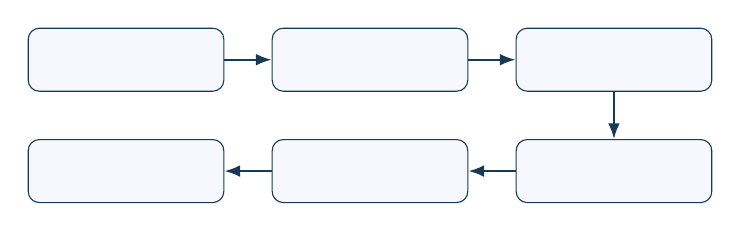
\begin{tikzpicture}[node distance=6mm]
\node[causalbox,text width=2.25cm] (q) {固定问题\\总体与时间};
\node[causalbox,text width=2.25cm,right=of q] (d) {模拟设计\\资格与分配};
\node[causalbox,text width=2.25cm,right=of d] (i) {识别审计\\假设与支持};
\node[causalbox,text width=2.25cm,below=of i] (e) {估计与诊断\\平衡与权重};
\node[causalbox,text width=2.25cm,left=of e] (s) {敏感性\\替代结构};
\node[causalbox,text width=2.25cm,left=of s] (a) {行动解释\\效用与边界};
\draw[causalarrow] (q)--(d);\draw[causalarrow] (d)--(i);\draw[causalarrow] (i)--(e);
\draw[causalarrow] (e)--(s);\draw[causalarrow] (s)--(a);
\end{tikzpicture}
\end{center}

\paragraph{把诊断改写为分析决策}

诊断的价值在于它会改变分析，而不是为附录增加一张图。若倾向得分两组几乎不重叠，预先规定的动作应是收缩目标人群、收集新对照或改用部分识别，不是不断更换分类器。若加权后平衡仍差，应修订处理模型或不再使用该权重。若负对照结果显示强关联，应将未测混杂纳入主结论的不确定性，而不是把它降格为“补充分析”。

同样，估计器之间的差异需要触发解释。在相同目标下，g计算、IPW与AIPW若结果接近，只表示对这些建模选择不敏感；若差异很大，需检查外推、极端权重和函数形式。不能从三个结果中选一个最显著的作为“主模型”。

\begin{failurecheck}[有效样本量与原始行数混为一谈]
假设原始数据有5000人，但少数未处理的高风险患者获得很大权重，使$n_{\mathrm{eff}}$只有450。报告“样本量5000”会让读者误以为每个反事实区域都有充足信息。应同时给出原始行数、独立分配单位数、权重后有效样本量和每个关键层的实际对照数。若信息单位是医院而不是患者，还应把医院数放在推断首位。
\end{failurecheck}

\paragraph{从单一区间到分层不确定性}

对上述住院案例，主表可报告ATE的抽样区间，但还应有三类另行结果。第一类是目标敏感性：把“七日内进入”改为“十四日内进入”，结局和处理含义如何改变。第二类是结构敏感性：未测病情需要多强才会将风险差推回零。第三类是迁移敏感性：项目从大型医院进入基层机构时，依从、容量和对照治疗是否保持。这些问题不宜被合成一个更宽的置信区间，因为它们来自不同证成来源。

\subsection{有限样本推断：随机性来自哪一层}

标准误不是估计器名称的固定配件。它要描述的是，在什么重复过程中，当前估计会如何变动。随机试验中可以把处理分配当作随机性来源；从超总体抽样时可把单位抽样当作来源；固定区县的全部医院数据则未必有一个明确的医院超总体。同一个数字在不同重复概念下可以有不同方差。

\begin{center}
\small
\begin{tabularx}{\textwidth}{>{\bfseries}p{2.4cm}X X}
\toprule
数据生成结构 & 不可拆分的信息单位 & 推断与重抽样原则\\
\midrule
个人随机试验 & 单个受试者，但要保留分层分配 & 按随机化设计或预先指定的稳健方差\\
整群随机试验 & 被随机化的学校、医院或社区 & 在群层重排处理，方差反映群数\\
重复测量 & 同一人的完整时间轨迹 & 按人划分训练折和bootstrap，不拆行\\
匹配或带放回对照 & 匹配组与被重复使用的单位 & 保留匹配及权重依赖，不当作独立两组\\
空间或网络数据 & 由溢出与同一冲击连接的单位 & 由设计定义暴露和分配，不只换用稳健标准误\\
\bottomrule
\end{tabularx}
\end{center}

例如一项学校级干预有30所学校、每校200名学生。若处理在学校层随机分配，6000行记录不能提供6000次独立处理比较。学校内教师、同伴和实施使结局相关；自由度与有效信息更接近30个群。普通个人级bootstrap会在每所学校内抽出大量看似新的独立单位，系统性低估方差。

\paragraph{小样本中稳健方差也会失效}

“使用群稳健标准误”只是开始。群数很少、群规模差异很大或处理群比例失衡时，常用大样本近似仍可能给出过窄区间。可根据设计使用群层随机化检验，使用小样本自由度修正，或者在有限数量匹配群内做精确重排。如果只有两个处理医院和两个对照医院，无论患者数多少，对普遍医院效应的统计推断都很脆弱。

随机化推断也不会自动解决处理后失访、不依从和干扰。它使用已知分配机制评估特定零假设；当结局只在选择后的人中观测，接受的处理版本因人而异，或一人的分配影响他人时，目标和估计方法都要重新定义。

\paragraph{多次交叉拟合与分割不确定性}

在样本不大时，一次随机分折可使某些稀少层几乎只落在一个训练集或评价集，导致DML与AIPW结果随随机种子明显变化。可重复若干次按处理与关键层分层的交叉拟合，报告各次点估计、标准误与最终汇总规则。重复分割不是为了在许多结果中选一个最有利数字，而是暴露训练样本选择对有限样本结果的影响。

需要注意，把多次分割的点估计标准差直接当作总标准误也不正确。每次估计仍共享同一原始样本，分割变动只是算法不稳定的一部分。最终区间应基于目标估计的影响函数或相应理论，并将分割范围作为附加诊断报告。

\begin{failurecheck}[随机拆行制造了虚假外样本]
电子健康记录中同一患者有多次就诊，若按行随机分到训练折和验证折，模型可以通过诊断组合、时间模式甚至隐式标识识别同一人。验证折不再表示新患者。更严重的是，后期就诊包含早期处理及结局的后果，会把处理后信息泄漏到基线预测。分折必须在因果单位与时间零点上完成，并在多中心数据中考虑是按患者、机构还是未来时段检验外推。
\end{failurecheck}

\begin{chapterreview}
识别之后仍可用多种估计器。g计算建模结果，匹配强调设计，IPW建模处理赋值，AIPW与TMLE结合二者，DML以正交得分和交叉拟合容纳高维学习。任何方法都必须与目标量、重叠和研究设计配套；置信区间只覆盖部分不确定性，诊断和敏感性分析不可省略。
\end{chapterreview}

\begin{selfcheck}
\begin{enumerate}
  \item 为什么处理模型的分类准确率不是倾向得分质量的主要标准？
  \item 解释AIPW的两部分分别承担什么功能，“双重稳健”不保证什么？
  \item 交叉拟合与Neyman正交性分别解决哪类机器学习偏差？
  \item 为一项观察研究设计包含重叠、平衡和敏感性分析的报告清单。
\end{enumerate}
\end{selfcheck}

\chapterreadings{
倾向得分的经典论文是\textcite{rosenbaumrubin1983}，应用诊断可读\textcite{austin2011}，匹配估计理论见\textcite{abadieimbens2006}。双重稳健的经典说明见\textcite{bangrobins2005}；潜在结果估计的系统处理见\textcite{imbensrubin2015}；观察性纵向方法见\textcite{hernanrobins2020}；TMLE见\textcite{vanderlaanrose2011}；DML的正式框架见\textcite{chernozhukov2018}。随机试验中的回归调整见\textcite{lin2013}，有限样本和聚类方差问题可结合\textcite{mackinnonwhite1985}与\textcite{cameronmiller2015}阅读。

匹配与分层的历史基础可由\textcite{cochran1968}和\textcite{rubin1973}追溯，现代方法综述见\textcite{stuart2010}；平衡诊断不应被倾向得分模型的预测精度替代，具体比较见\textcite{austin2009}。估计倾向得分的效率结果见\textcite{hirano2003}，直接以平衡为目标的加权和估计可对照\textcite{li2018}与\textcite{imairatkovic2014}。

缺失协变量下的影响函数与加权基础见\textcite{robins1994}，TMLE的原始学习框架见\textcite{vanderlaanrubin2006}。重叠不足时应改变目标或样本而非依赖外推，见\textcite{crump2009}；小样本稳健标准误的有限样本问题见\textcite{imbenskolesar2016}。未测混杂敏感性可分别从非参数界限\parencite{dingvanderweele2016}与回归遗漏变量解释\parencite{cinellihazlett2020}进入。
}


\part{发现、迁移、机器学习与应用}
\input{chapters/chapter-08-discovery}
\chapter{外部效度、可迁移性与数据融合}
\label{ch:transportability}

\begin{learninggoals}
读完本章，你应当能够：区分样本代表性、效应修饰与形式可迁移性；使用标准化、加权和选择图组织跨总体推断；审查重叠、测量协调、制度变化与系统反馈。
\end{learninggoals}

\section{外部效度、可迁移性与数据融合}

\subsection{目标人群、标准化与变量选择}

一项随机试验可以在入组样本中无偏估计治疗效应，却不能仅凭随机化说明结果适用于未入组者。\term{内部效度}关心样本内处理比较是否有效；\term{外部效度}关心结论能否适用于其他人群、地点、时间或干预版本。
文献中常区分\term{普遍化}（目标人群包含试验样本）与\term{迁移}（试验样本和目标人群可能来自不同总体），但术语使用并不完全统一。更重要的是明确两个域：源域 $S=1$ 提供何种实验或观测数据，目标域 $S=0$ 要回答哪个因果目标，它们在哪些机制上不同。
平均效应不是处理的固定属性。若治疗效果随年龄、基线风险、医疗资源或依从策略变化，样本构成改变就会改变ATE。外推因此不是在结果末尾加一句“需要更多研究”，而是一个可以建模的因果问题。

\paragraph{从样本效应到目标人群效应}

设试验中处理随机化，$S=1$ 表示进入试验，目标为整个目标人群中的 $E\{Y(a)\}$。若给定基线协变量 $L$ 后，潜在结果与入组状态可交换：
\[
Y(a)\indep S\mid L,
\]
并且试验与目标人群在相关 $L$ 上都有支持，则
\[
E\{Y(a)\}=\sum_l E(Y\mid A=a,S=1,L=l)P(L=l).
\]

右侧用试验估计每个 $L$ 层的处理结果，用目标人群的 $L$ 分布重新标准化。若目标只包含 $S=0$ 的非试验成员，则权重分布换成 $P(L\mid S=0)$。这与内部效应的混杂调整形式相似，但可交换对象不同：内部效度要求处理组可比，迁移要求源域与目标域在给定效应相关变量后可比。
选择概率加权提供等价实现。试验中较少代表目标人群的单位获得较大权重。与处理权重一样，接近零的试验参与概率产生极端权重；若目标人群包含试验从未覆盖的协变量组合，非参数迁移不可识别。

\paragraph{哪些变量需要用于迁移}

不是所有预测结果的变量都是\term{效应修饰因子}。一个变量可以强烈预测未治疗风险，却不改变绝对处理效应；也可能在风险比尺度上无修饰、在风险差尺度上有修饰。迁移变量的选择依赖效应尺度与结构。
理想集合应阻断选择 $S$ 与潜在结果之间导致效应差异的路径。纳入基线结局预测因子常有稳健性收益，但过度细分会破坏重叠。若一个未测变量同时影响入组和处理反应，单靠已测人口学标准化仍不足。
机制知识在这里特别重要。若药物通过某受体发挥作用，而受体分布在两域不同，受体或其可靠代理是迁移关键；若两域只在与效果无关的行政变量上不同，无需为表面代表性调整。样本“看起来像”目标人群不是充分标准。

\subsection{选择图、多源融合与时间变化}

Pearl与Bareinboim用\term{选择图}在因果图上增加选择节点，标记哪些机制可能跨域变化\parencite{pearlbareinboim2014}。若 $S_X\rightarrow X$，表示 $X$ 的生成机制在源域与目标域不同；没有选择节点指向某变量，则假定其条件机制稳定。

假设源域有 $X$ 的随机试验，目标域只有观测数据，且选择只影响中介前的协变量 $Z$。若在适当干预图中
\[
Y\indep S\mid Z,\doop(X),
\]
则 $Z$ 是对迁移\term{S-可容许}的：源域中按 $Z$ 分层的实验效应可用目标域 $P(z)$ 加权。

更复杂情形可用do-calculus与选择节点推导\term{迁移公式}。某些目标域机制虽然变化，却能由目标观测数据直接估计；稳定的干预关系则从源实验带入。可迁移性因此不是要求两域完全相同，而是要求差异的位置已知且可由可用数据桥接。

\paragraph{多源数据融合}

现实证据可能包括一个小型随机试验、大型电子病历、多个国家调查和机制实验。\term{数据融合}寻求组合各源的互补信息：试验提供处理赋值的内部效度，观察数据提供目标人群分布、长期结局或稀有亚组。

融合前必须统一：

\begin{itemize}
  \item 变量定义与测量尺度；
  \item 时间零点、随访和删失规则；
  \item 处理版本与依从策略；
  \item 每个数据源的选择机制；
  \item 哪些结构方程被假定跨源稳定。
\end{itemize}

同名变量不保证同一构念。不同医院的“重症”可能由不同编码规则产生；不同国家的教育年限代表不同课程质量。若测量机制跨域变化，直接把变量视为共同节点会把测量差异误作因果异质性。
融合也可能降低而非提高可信度。一个内部偏差严重的大数据集会以高精度支配结果；贝叶斯或加权整合若没有明确偏差模型，只是把不相容来源平均。应先写出每个来源为哪个目标提供何种识别信息，再决定组合。

\paragraph{时间迁移与政策改变}

从过去迁移到未来不仅是协变量再加权。诊断技术、背景治疗、行为响应和制度规则可能改变因果机制本身。COVID-19早期治疗效果无法仅按年龄结构加权到后期，因为病毒变体、免疫背景和标准护理同时变化。
政策还可能改变系统均衡。小规模补贴试验估计的是部分覆盖时的个体反应，全国推广会改变价格、劳动力供给和社会规范。SUTVA下的个体效应无法直接迁移到不同政策饱和度。应把覆盖率、网络或市场状态纳入处理定义，或使用结构经济模型与干扰设计。

\subsection{敏感性、数值标准化与测量协调}

迁移假设通常比样本内随机化更难验证。可以进行：

\begin{itemize}
  \item 比较源域和目标域的协变量支持与参与概率；
  \item 在源域内部留出子群，检验迁移方法能否恢复已知结果；
  \item 对未测效应修饰因子的分布和交互强度设定情景；
  \item 比较多个效应尺度和处理版本；
  \item 使用目标域中的负对照或短期可观测结局检查机制稳定性；
  \item 若缺乏重叠，报告目标子人群或部分识别界限。
\end{itemize}

外部效度不应以“样本是否人口学代表”二元判断。一个非代表性样本在测得关键效应修饰因子并有良好重叠时可以迁移；一个表面代表样本若处理、测量或机制与目标应用不同，仍可能不适用。

\paragraph{数值例子：同一分层效应，不同总体效应}

设试验中年轻人占80\%、老年人占20\%；治疗使年轻人风险下降2个百分点，使老年人下降10个百分点。试验ATE为
\[
0.8\times(-0.02)+0.2\times(-0.10)=-0.036.
\]
目标人群年轻人与老年人各占一半，则在分层效应可迁移时，目标ATE为
\[
0.5\times(-0.02)+0.5\times(-0.10)=-0.06.
\]
试验内部估计没有错，直接搬用 $-3.6$ 个百分点却回答了错误人群。

若年龄只是基线风险预测因子，而风险差在两层相同，重新加权不会改变风险差；在风险比尺度上却可能因基线风险不同出现另一表现。因此效应修饰和迁移必须指定尺度。一个变量是否“必须调整”不能脱离目标尺度宣布。
若目标人群包含试验中完全没有的90岁以上人群，公式要求的分层结果不存在。用回归平滑外推不是非参数识别，而是增加关于年龄---效应曲线的模型。报告应把重叠内标准化与重叠外模型外推分开。

\paragraph{测量协调的因果含义}

两个数据源都含“血压”，源域使用诊室单次测量，目标域使用家庭一周均值。二者误差结构和对白大衣效应的敏感度不同。若把它们当同一 $L$，选择差异可能其实是测量差异；若血压用于识别效应修饰，错误会破坏迁移可交换性。
协调可使用验证子样本中同时测两种指标，建立测量桥接模型；也可把潜在真实血压和两个测量节点显式画出。简单z分数标准化只统一单位与边际分布，不证明构念等价。
结局也需协调。一个系统用住院编码，另一个用临床判定；治疗还可能改变就医概率。外推时必须区分真实疾病机制是否稳定与结局观测机制是否稳定。选择图可以分别把选择节点指向潜在结局和测量节点。

\paragraph{迁移失败诊断与公平责任}

若加权后的源域能复现目标域中处理前或已知短期关系，却无法复现目标结局，可能有三种原因：遗漏效应修饰、处理或结局定义不一致、结果机制真实变化。仅继续增加人口学权重无法区分。
可使用“桥接结果”：选择在两域都观察、对机制变化敏感的中间结局，检查模型；使用多源实验比较同一分层效应；或在目标域开展小型校准试验。若少量目标实验与大源试验不一致，可用分层模型估计变化，而非强行假定完全相同。
运输公式的失败也是信息：它指出哪个机制需要目标域数据。最有价值的新样本不一定扩大总量，而可能专门覆盖缺失协变量层或直接测量疑似变化机制。

\paragraph{公平与外部效度}

训练与试验样本往往对边缘群体覆盖不足。总体平均效果良好可能掩盖某群体没有重叠或测量质量更差。以“总体可迁移”为唯一验收，会把不确定性集中到最缺乏证据的人。
报告应按政策相关群体展示支持范围、分层效应与迁移权重，不把极端权重产生的高方差估计包装为同等证据。必要时限制部署、优先收集目标群体数据，或采用保守决策界限。外部效度因此也有分配伦理：谁被纳入知识基础，会影响谁承担模型失败。

\section{从迁移公式到政策责任}

\subsection{迁移目标与选择图表达}

外部效度不是问研究“能否推广”这一笼统问题，而是定义目标总体中的效应。例如试验样本以$S=1$表示，目标总体以$S=0$表示，要估计
\[
E\{Y(1)-Y(0)\mid S=0\}.
\]
若给定处理前变量$X$后，试验参与与潜在结果独立，并且目标总体中的每类$X$在试验中都有支持，则可用试验内条件效应按目标分布标准化。随机化解决试验内部处理比较，参与交换性和参与正值性则连接试验与目标，两者缺一不可。

需要迁移的变量是效应修饰和选择机制的交集，而非所有结局预测因子。一个强预测因子若不改变处理效应，试验与目标分布不同不会造成平均效应差；一个弱边际预测因子却可能强烈修饰效应。领域知识、分层试验结果和机制证据共同决定变量选择，纯粹用预测重要性排序会偏离目标。
目标总体也可能随时间变化。把十年前试验迁移到今天，不只是年龄和疾病分布变化，治疗标准、诊断阈值、竞争风险和实施能力都可能改变。时间应作为环境机制的一部分，而非仅在回归中加入年份。

\paragraph{选择图怎样组织跨域差异}

选择图用特殊节点指向在源域和目标域之间可能改变的机制。若选择节点只指向基线变量$X$，而$Y$的结构机制给定$A,X$后稳定，可以通过目标域$P(X)$与源域试验条件效应组合。若选择直接指向$Y$，说明结果机制存在未由测量变量解释的变化，简单重加权通常不足。
图的价值是区分分布变化与机制变化。人口年龄结构改变属于输入分布变化；同样治疗在新医院因执行质量不同而改变效果，属于处理或结果机制变化；结局编码系统改变则是测量机制变化。三者可能产生相似的观测差异，却需要不同修复：重加权、重新校准实施模型或做测量桥接研究。
多源数据融合可让不同数据源贡献不同模块。随机试验提供处理到结果的内部效应，登记数据提供目标协变量分布，机制研究约束中介路径，政策数据库提供环境差异。但来源之间必须有共同变量语义和可连接单位；若“严重度”在各库中定义不同，形式上的同名节点不能直接拼接。

\subsection{测量协调与规模效应}

跨域研究常把测量差异当作数据清洗问题。实际上测量过程可能决定因果目标。试验中的抑郁结局由临床访谈获得，目标系统只有处方记录；二者不仅噪声大小不同，还可能测量不同构念。若处理影响求医和处方机会，处方记录甚至是处理后选择变量。
协调应建立构念---指标图：先定义希望比较的潜在构念，再记录每个数据源的观测指标、阈值、测量时点和缺失机制。可以使用共同样本、校准研究、潜变量模型或多指标设计建立桥梁，但每种方法都增加假设。没有桥接数据时，把变量重命名为同一英文缩写不会创造可比性。
处理也需要协调。一个试验的“常规照护”可能包含频繁随访，目标地区的常规照护几乎没有服务；药物剂量、供应、依从支持和共同治疗都会改变版本。迁移结论应针对完整策略，并说明哪些组成部分被假定等价。

\paragraph{规模扩大为何可能改变效应本身}

小规模试验通常把资源价格、人员行为和网络环境视为背景不变。全面部署会改变这些背景：培训需求降低执行质量，补贴推高价格，推荐系统改变内容供给，疫苗覆盖产生群体免疫。个体潜在结果因此依赖总体处理比例或网络配置，简单把试验平均效应乘以人口规模会失败。
处理这种问题需要定义饱和度或政策水平。可比较不同集群覆盖率下的直接效应与溢出效应，或建立供需和网络传播模型。外推对象不再是“同一个体处理从0变1”，而是整个系统从一种配置转向另一种配置。识别需要集群随机化、分阶段实施或结构模型，并清楚说明均衡假设。
规模效应也可能改变受益者组成。试点期最有动机、最易服务的人先参与，扩展后进入边缘群体；早期执行者经验丰富，后期机构能力较弱。监测部署过程应持续更新目标总体、实施版本和支持区域，而不是把一次外部效度分析视为永久许可证。

\paragraph{外部效度的分配责任}

哪些人进入试验、哪些结局被测量、哪些亚组有足够支持，会决定谁能从证据中受益。若弱势群体长期被排除，模型对他们的不确定性更高；按预测置信度分配资源又可能进一步排除他们，形成证据贫困循环。外部效度因此不仅是技术准确性，也是研究资源的分配问题。
负责任的报告应展示目标群体覆盖、重叠和分层不确定性，不用总体平均掩盖支持缺口。部署可以采用分阶段策略：在证据充分群体中先实施，在缺口群体中同步开展有保护措施的研究；也可以使用保守决策界限，避免把高方差外推包装成个性化精确。
价值判断还进入目标选择。最大化总体平均收益可能牺牲小群体，最小化最坏群体风险则可能降低平均效率。统计模型不能独自选择公平准则，但可以明确不同准则需要哪些效应、成本和不确定性信息，使规范分歧不再隐藏在默认损失函数中。

\section{迁移分析的计算、诊断与治理}

\subsection{标准化计算与普遍化诊断}

设试验中低风险层占80\%，处理效应为风险下降2个百分点；高风险层占20\%，处理效应为下降10个百分点。试验平均效应是$0.8\times(-0.02)+0.2\times(-0.10)=-0.036$。目标人群若低风险占30\%、高风险占70\%，标准化效应为$0.3\times(-0.02)+0.7\times(-0.10)=-0.076$。
两个数值都正确，却回答不同总体。差异不是试验“失去内部效度”，而是效应修饰与人群组成共同作用。若只报告相对风险，而基线风险也跨域变化，绝对收益差异可能更大。迁移报告应同时展示分层效应、源域与目标分布以及加权后的总体结果。
如果目标高风险层在试验中完全没有样本，上式中的$-0.10$无法由试验估计。用回归预测出的数值依赖外推模型；应限制目标、补充试验或给出基于机制与外部数据的范围。正值性诊断比权重公式更先决定结论可信度。

\paragraph{试验普遍化的诊断顺序}

第一步比较资格标准：哪些目标成员原则上不能进入试验，排除是否与效应修饰相关。第二步比较参与倾向与协变量分布，展示试验和目标中的重叠。第三步检查处理、结局和随访是否同义。第四步估计参与权重或标准化模型，并报告权重分位数与有效样本量。第五步使用替代变量集、截尾和结果模型检查敏感性。
诊断不能只看加权后基线均值。参与模型可能在边缘群体外推，结局机制可能跨机构变化，未测效应修饰仍存在。可利用目标域观测结局、不同试验或负对照环境检查模型，但这些数据也有自身混杂。最可靠的结论会明确哪些差异已由数据桥接，哪些仍由稳定性假设承担。
普遍化与可迁移性有时区分为目标总体是否包含试验样本，但实质逻辑相近：都是把源域条件关系与目标域分布组合。术语选择不应遮蔽共同的交换与支持条件。

\subsection{证据冲突与部署后审计}

两个试验给出不同效果，可能因人群、剂量、对照、结局或执行质量不同，也可能只是抽样波动。数据融合前应建立差异表，而不是立即做一个加权平均。若差异可由测量的效应修饰解释，可分别标准化到共同目标；若处理版本不同，应保留为不同策略；若结果机制直接变化，层次模型的“研究随机效应”只能描述异质，不能解释可迁移性。
观察研究与试验冲突时，试验在内部处理比较上通常更强，但观察研究可能覆盖长期、罕见结局和不同实施环境。应检查试验依从、失访和结局时窗，同时对观察研究做偏差分析。冲突可生成新的目标：短期生物效应是否稳定，而长期政策效应为何随系统改变。
证据综合的输出可以是分层结论，而非单一数值。例如对试验覆盖人群给出较窄效应，对外推人群给出宽范围，对新实施版本暂不量化。这样的结构比一个忽略来源差异的总体元分析更适合决策。

\paragraph{部署后的持续迁移审计}

迁移不是发布前一次性步骤。部署会改变参与者、执行者和环境，原有目标分布不断更新。系统应监测处理版本、关键效应修饰、重叠、结局测量和策略依从；当这些指标越过预定阈值，触发重新估计、局部试验或暂停外推。
结果监测要避免选择反馈。政策决定谁接受处理，接受又决定谁产生标签；只比较部署后处理组与未处理组会重现混杂。可保留小比例随机探索、使用分阶段推广或设计可信的准实验。若伦理上不能随机，应至少保存完整决策日志和处理概率，为离策略评价提供依据。
模型退役也是迁移治理的一部分。新治疗替代旧对照、编码体系改变或关键群体缺乏支持时，应明确结束旧结论的适用期，而不是无限再校准。证据有生命周期，外部效度报告应包含下一次审查条件。

\subsection{完整迁移案例：从专科试验到城市系统}

某专科中心完成了一项康复项目随机试验，现在城市医疗系统想判断全面推广后的一年住院风险差。$S=1$表示进入试验，$S=0$表示只在目标总体登记；$A$为康复项目，$Y$为住院，$L$包含基线风险与行动能力。试验保证$S=1$中$A$的可交换性，却不保证试验参与者与城市患者拥有相同结局机制。

\begin{center}
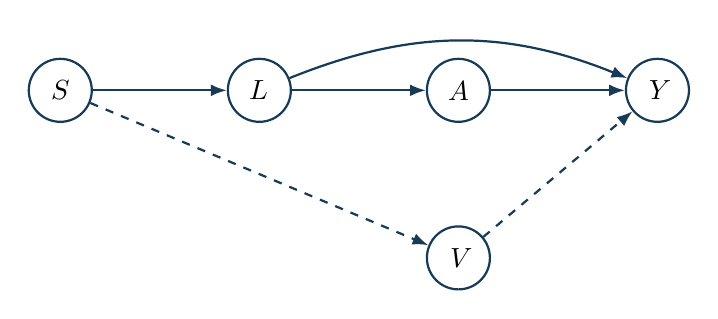
\begin{tikzpicture}[node distance=13mm and 17mm]
\node[causalnode] (s) {$S$};
\node[causalnode,right=of s] (l) {$L$};
\node[causalnode,right=of l] (a) {$A$};
\node[causalnode,right=of a] (y) {$Y$};
\node[causalnode,below=of a] (v) {$V$};
\draw[causalarrow] (s)--(l);
\draw[causalarrow] (l)--(a);\draw[causalarrow] (l) to[bend left=22] (y);
\draw[causalarrow] (a)--(y);
\draw[causalarrow,dashed] (s)--(v);\draw[causalarrow,dashed] (v)--(y);
\end{tikzpicture}
\end{center}

实线部分表示，试验招募使$L$的分布不同，而$L$修饰处理效应。若给定$L$后潜在结果可在试验与目标间交换，且目标每个$L$层都在试验有支持，则
\[
E{Y(a)\mid S=0}=
\sum_l E(Y\mid A=a,L=l,S=1)P(l\mid S=0).
\]
虚线部分表示一个更强风险：实施容量$V$在专科中心与城市系统中不同，并直接影响$Y$。若$V$没有测量，只对$L$标准化无法修复机制变化。这不是权重模型的小误差，而是小规模试验中的“每人每周两次指导”与全市推广时的处理版本已经不同。

\begin{workedexample}[总体组成改变的数值后果]
将$L$分为可独立行走和行动受限两层。试验分别估计的住院风险差为$-0.08$与$-0.18$。试验中两层占比为0.75和0.25，因而试验平均为
\[
0.75\times(-0.08)+0.25\times(-0.18)=-0.105.
\]
城市目标中两层占比为0.35和0.65，若分层效应可迁移，目标平均为
\[
0.35\times(-0.08)+0.65\times(-0.18)=-0.145.
\]
差异来自效应修饰与总体组成，不是试验随机化失效。但若城市中还有“需他人协助行走”而试验完全排除的第三层，该层效应不能由两个已观察数字插值。必须限定目标、补充试验或给出外推范围。
\end{workedexample}

\paragraph{参与权重的解释与诊断}

当试验参与可由$L$解释时，可为试验中的人赋予与其在目标中代表性成比例的权重。一种参与几率权重与
\[
\frac{P(S=0\mid L)}{P(S=1\mid L)}
\]
成比例。它使试验中稀少、目标中常见的行动受限者获得更大代表性。权重并不证明这些人与未参加者在所有效应修饰上相同；它只实施已写出的可迁移假设。

诊断应先分层回答三个问题。第一，目标中有哪些人几乎不可能进入试验？第二，大权重是因为少数合理的稀有类型，还是参与模型函数形式不稳定？第三，加权后已测$L$是否与目标分布对齐？应报告权重分位数、有效样本量、每个目标层的试验人数和截尾后目标的变化。

\paragraph{测量协调先于数值融合}

专科中心可能以专业评定表测量行动能力，城市登记系统却只有辅具申请和诊断编码。即使两边都有一个名为“行动限制”的二元变量，切点、记录动机和测量时点不同也会使标准化失真。应先建立变量映射表，报告可互换、需校准和无法对齐的字段；再用重叠子样本或验证研究估计测量桥接。

结局测量也需同样审查。试验中的住院由独立委员会裁定，目标数据中则来自医保结算；跨市就医或康复项目对就医行为的改变会造成差异漏报。若测量误差受$A$或$S$影响，它不是简单降低精度，而会改变迁移查询的含义。

\begin{center}
\small
\begin{tabularx}{\textwidth}{>{\bfseries}p{2.1cm}X X}
\toprule
风险层 & 可观测诊断 & 应对动作\\
\midrule
总体支持 & 目标层在试验无或极少样本 & 限定目标、补充招募或报告外推范围\\
效应修饰 & 分层效应差异且人群组成改变 & 按目标分布标准化并报告分层结果\\
测量协调 & 字段同名但时点、切点或来源不同 & 建立映射与验证子研究\\
实施版本 & 容量、依从或对照治疗跨域变化 & 改写处理策略并进行局部试验\\
系统反馈 & 覆盖率扩大后等待、价格或行为变化 & 监测饱和度并使用分阶段部署\\
\bottomrule
\end{tabularx}
\end{center}

\begin{failurecheck}[把内部效度高写成全部人群可用]
随机化使试验内的处理比较可信，但不回答目标中缺失的效应修饰、处理版本或规模效应。“高质量RCT已证明有效”至少应拆成三句：试验内哪个策略比较被识别，目标总体与试验差异由哪些变量桥接，全面部署是否保留相同干预与结局机制。任何一句缺少时，数值都应带有相应的限定。
\end{failurecheck}

\subsection{多源数据融合：每个来源只提供它识别的部分}

现实中常没有一份数据同时包含随机处理、长期结局、代表性人群和完整测量。数据融合的任务不是把所有行连接成一张大表，而是明确每个来源识别哪个因子或桥接关系。例如，随机试验可识别短期处理效应，城市登记可提供目标协变量分布与长期结局，一个小型验证子研究可连接两种测量标尺。

\begin{center}
\small
\begin{tabularx}{\textwidth}{>{\bfseries}p{2.2cm}X X}
\toprule
数据来源 & 主要可提供的信息 & 不能单独提供的信息\\
\midrule
专科中心RCT & 已定义处理版本下的内部处理比较 & 全市人群组成、大规模实施效应\\
城市登记 & 目标总体分布、常规实施与长期结局 & 无未测混杂的处理效应\\
测量验证子研究 & 专业评定与登记代理之间的误差桥接 & 处理效应与系统规模反馈\\
部署试点 & 目标环境中的依从、容量、安全与短期效果 & 未试点地区的无条件长期效应\\
\bottomrule
\end{tabularx}
\end{center}

一个可识别的融合式必须对这些信息接口有明确要求。例如要用RCT的短期行动改善$M$与登记中$M$到长期住院$Y$的关系推断$A$到$Y$，需要$M$足以中介处理的长期影响，登记中$M-Y$关系可在测量的共同原因后交换，且试验与登记中$M$的测量可比。任何一项都比“两个数据集样本大”更重要。

\paragraph{证据冲突要先对齐估计对象}

假设RCT报告风险差$-0.10$，登记调整研究为$-0.04$，部署试点为$-0.07$。不能先假定三个数字在估计同一个常数真值。应分别列出资格、处理版本、对照水平、随访时窗、结局尺度与效应人群。若RCT为密集专业康复，登记的处理为“至少一次转诊”，数值差异首先反映处理不同，而不是某一研究“错了”。

对齐后仍有冲突时，可把每个偏差方向显式化。专科试验依从较高，可能高估全面实施效果；登记中未测病情使重症者更容易接受康复，可能将保护效应向零拉；试点规模小，容量反馈尚未完全出现。这些方向不会自动告诉真值，但会指出需要的负对照、依从调查、容量实验与未测混杂敏感性参数。

\paragraph{规模改变会让干预本身内生变化}

在500人试验中，每位治疗师负责10人；全市推广后若仍只有50位治疗师，每人负责数上升、等待延长，项目实际剂量与质量会变化。此时不能说“个体效应不变，只是更多人参加”。覆盖率通过系统资源反过来改变处理版本。

可把治疗师负荷和等待时间放入干预描述，定义不同覆盖率下的总体效应；也可在不同地区分阶段提高覆盖率，直接学习饱和度反应。政策容量是因果变量，不是预算附注。对存在网络、市场与供给约束的系统，只估计低覆盖个体效应不足以支持全面部署。

\begin{failurecheck}[把数据源标签当作一个普通协变量]
在联合数据中加入“来源=RCT/登记”指示变量并拟合一个大回归，不会自动使两个数据生成机制可交换。来源节点可能同时改变招募、处理分配、结局测量与实施强度。应使用选择图或明确的数据融合假设分别标记哪些模块改变，再检查手中数据是否为每个改变提供桥接。
\end{failurecheck}

\begin{chapterreview}
内部效度不能自动保证外部效度。迁移把源域实验关系与目标域协变量分布或观测机制结合；选择图明确哪些机制跨域变化。可靠融合要求统一变量、时间和处理版本，并说明每个数据源提供的识别信息。效应修饰、重叠、测量变化和系统均衡是外推的核心限制。
\end{chapterreview}

\begin{selfcheck}
\begin{enumerate}
  \item 推导试验效应按目标人群协变量分布标准化的公式，并列出三项假设。
  \item 为什么强结局预测因子不一定是迁移所需的效应修饰变量？
  \item 为两个医疗系统画选择图，标出治疗、测量和基线风险的可能变化机制。
  \item 解释小规模政策试验推广到全国时，个体效应为何可能失效。
\end{enumerate}
\end{selfcheck}

\chapterreadings{
选择图与形式可迁移性见\textcite{pearlbareinboim2014}和\textcite{bareinboimpearl2016}。试验普遍化与加权方法可读\textcite{cole2010}、\textcite{stuart2011}和\textcite{westreich2017}；嵌套与非嵌套试验设计及其抽样含义见\textcite{dahabreh2019}与\textcite{dahabreh2021}。\textcite{degtiarrose2023}提供了外部效度方法的系统综述。将可迁移性置于目标试验框架中时，可结合\textcite{hernanrobins2020}。

形式可迁移性的一般判定算法见\textcite{bareinboimpearl2013}。基于倾向分层的试验普遍化见\textcite{tipton2013}，样本与总体相似度的量化诊断见\textcite{tipton2014}；不同推广估计器的模拟和经验比较可读\textcite{kern2016}。抽样权重在实际随机试验中的实现见\textcite{buchanan2018}，而\textcite{westreich2019}强调内部效度、目标效度和研究设计等级不能混为一谈。

跨地点预测政策效果的早期计量方案见\textcite{hotz2005}，教育干预普遍化方法的专题综述见\textcite{tiptonolsen2018}。这些文献应与正文的处理版本、重叠和规模反馈共同阅读，避免把统计重加权误当成机制自动稳定。

迁移不仅是抽样权重问题。从证据进入新政策环境所需的支撑因素见\textcite{cartwright2007}，随机试验为何不能仅凭设计标签保证外部适用性可对照\textcite{deatoncartwright2018}。
}

\input{chapters/chapter-10-causal-ml-applications}

\input{chapters/chapter-11-synthesis-open-problems}

\appendix
\part{专题附录与学习工具}
\input{chapters/appendix-A-comparative-topics}
\input{chapters/appendix-B-glossary-learning}
\input{chapters/appendix-C-exercises}
\input{chapters/appendix-D-primary-reading}

\backmatter
\printbibliography[heading=bibintoc,title=参考文献]
\cleardoublepage
\phantomsection
\addcontentsline{toc}{chapter}{主题索引}
\renewcommand{\indexname}{主题索引}
\printindex

\end{document}
